\documentclass[12pt,a4paper]{report}
\usepackage{geometry}
\geometry{a4paper, margin=2.5cm}

\usepackage[utf8]{inputenc}
\usepackage[T1]{fontenc}
\usepackage{mathptmx} % Times New Roman font for professional look
\usepackage{graphicx}
\usepackage{amsmath}
\usepackage{booktabs}
\usepackage{setspace}
\usepackage{parskip}
\usepackage{caption}
\usepackage{titlesec}
\usepackage{fancyhdr}
\usepackage[colorlinks=true, linkcolor=MidnightBlue, citecolor=MidnightBlue, urlcolor=MidnightBlue]{hyperref}
\usepackage[dvipsnames]{xcolor}
\usepackage{float}
\usepackage{multirow} % For complex tables

% Packages required for Engineering Graphs
\usepackage{tikz}
\usepackage{pgfplots}
\pgfplotsset{compat=1.18}

% Chapter and Section Formatting
\titleformat{\chapter}[hang]{\Huge\bfseries\color{MidnightBlue}}{\thechapter.}{20pt}{\Huge\bfseries}
\titlespacing*{\chapter}{0pt}{0pt}{40pt}
\titleformat{\section}{\Large\bfseries\color{MidnightBlue}}{\thesection}{1em}{}
\titleformat{\subsection}{\large\bfseries\color{MidnightBlue}}{\thesubsection}{1em}{}

% Header and Footer Formatting
\pagestyle{fancy}
\fancyhf{}
\fancyhead[L]{\textcolor{gray}{\small Engineering Marvels of Sri Lanka}}
\fancyhead[R]{\textcolor{gray}{\small NANO2162}}
\fancyfoot[C]{\thepage}
\renewcommand{\headrulewidth}{0.4pt}
\renewcommand{\footrulewidth}{0.4pt}

\begin{document}
	
	% =========================
	% PROFESSIONAL TITLE PAGE
	% =========================
	
	\begin{titlepage}
		
		\begin{center}
			
			% University Logo
			\vspace*{0.5cm}
			
\includegraphics[width=0.23\textwidth]{logo.jpg}
			
			\vspace{0.65cm}
			
			% University Name
			{\Large\bfseries WAYAMBA UNIVERSITY OF SRI LANKA}
			
			\vspace{0.25cm}
			
			% Department
			{\large Department of Nano Science Technology}
			
			\vspace{0.45cm}
			
			% Top Divider
			\textcolor{MidnightBlue}{\rule{\textwidth}{1.2pt}}
			
			\vspace{0.65cm}
			
			% Main Title
			{\fontsize{24}{29}\selectfont
				\bfseries ENGINEERING MARVELS \vspace{1cm} OF SRI LANKA}
			
			\vspace{0.65cm}
			
			% Bottom Divider
			\textcolor{MidnightBlue}{\rule{\textwidth}{1.2pt}}
			
		\end{center}
		
		% Space before submission information
		\vspace{4.8cm}
		
		% Submission Information
		\noindent
		\begin{minipage}[t]{0.47\textwidth}
			\raggedright
			
			{\large\bfseries Submitted to:}
			
			\vspace{0.18cm}
			
			{\normalsize Dr. Ashane Fernando}
			
			\vspace{0.12cm}
			
			{\normalsize Module: NANO2162}
			
		\end{minipage}
		\hfill
		\begin{minipage}[t]{0.47\textwidth}
			\raggedleft
			
			{\large\bfseries Submitted by:}
			
			\vspace{0.18cm}
			
			{\normalsize Group No: 12}
			
			\vspace{0.12cm}
			
			{\normalsize
				249152 / 249179 / 249110 / 249236}
			
		\end{minipage}
		
		% Push date to bottom
		\vfill
		
		\begin{center}
			
			{\large\bfseries Date of Submission}
			
			\vspace{0.18cm}
			
			{\normalsize 30 August 2026}
			
		\end{center}
		
		\vspace{0.35cm}
		
	\end{titlepage}
	
	\setcounter{page}{1}
	
	\chapter*{Executive Summary}
	\addcontentsline{toc}{chapter}{Executive Summary}
	
	Sri Lanka possesses a rich history of engineering that spans thousands of years, evolving from ancient hydraulic systems and colossal masonry to modern massive dams and railway bridges. This comprehensive report explores five of the most significant engineering marvels in Sri Lanka: the Sigiriya Rock Fortress, Jetavanaramaya Stupa, Jaya Ganga, Nine Arches Bridge, and the Victoria Dam. Moving far beyond traditional historical descriptions, this document systematically categorizes each marvel into its historical background, advanced material properties, dynamic engineering challenges, and profound structural significance.
	
	By integrating rigorous mathematical models, hydrostatic force integrations, structural stress-strain graphs, and real-world geotechnical parameters, this report critically analyzes these structures through the lens of modern engineering physics. Crucially, recognizing the scope of Nano Science Technology (NANO2162), this document establishes how the inevitable degradation of these structures—caused by material fatigue, micro-cracking, and capillary water absorption—can be combated using cutting-edge nanotechnological conservation methods, such as nano-silica consolidants and self-healing bio-concrete matrices.
	
	\newpage
	\tableofcontents
	\newpage
	\listoffigures
	\addcontentsline{toc}{chapter}{List of Figures}
	\newpage
	\listoftables
	\addcontentsline{toc}{chapter}{List of Tables}
	\newpage
	
	\pagenumbering{arabic}
	\setcounter{page}{1}
	\onehalfspacing
	
	%=========================================
	% CHAPTER 1: INTRODUCTION
	%=========================================
	\chapter{Introduction}
	The island nation of Sri Lanka boasts an exceptional engineering heritage that demands rigorous technical scrutiny to be fully appreciated. Early Sri Lankan civilizations were masters of hydrology, applied material science, and structural engineering, creating monumental architecture and irrigation networks that rivaled global wonders \cite{wijesuriya1998}. However, unlike structures built primarily on solid limestone bedrock in arid climates—such as the Great Pyramids—Sri Lankan engineers conquered complex tropical clay soils, extreme wind shears, and torrential monsoonal climates \cite{cooray1984}. 
	
	This report investigates five outstanding engineering achievements, shifting the paradigm from historical awe to critical technical evaluation. Each marvel is analyzed under a strict framework:
	\begin{itemize}
		\item \textbf{Historical Background:} The socio-political drivers behind the construction.
		\item \textbf{Construction Materials:} The chemical and physical properties of the ancient and modern materials utilized.
		\item \textbf{Engineering Challenges:} The logistical, geographical, and mechanical obstacles overcome by the builders.
		\item \textbf{Engineering Significance:} The mathematical and physical brilliance of the structural design.
	\end{itemize}
	
	Furthermore, in alignment with the Nano Science Technology curriculum, this report addresses the critical vulnerabilities of these aging structures and proposes modern nanotechnological interventions for their sustainable conservation.
	
	%=========================================
	% CHAPTER 2: SIGIRIYA
	%=========================================
	\chapter{Sigiriya Rock Fortress}
	
	\section{Historical Background}
	Constructed during the reign of King Kasyapa (477 – 495 CE), Sigiriya is a 200-meter-high sheer gneiss monolith transformed into a heavily fortified citadel and a sprawling urban complex \cite{bandaranayake1974}. Transforming this massive rock into an impenetrable fortress while maintaining aesthetic luxury required unprecedented advancements in hydrodynamics and structural keying.
	
	\section{Construction Materials and Degradation}
	The construction heavily utilized the natural \textit{Gneiss} bedrock. Millions of locally fired clay bricks were used for retaining walls. The famous "Mirror Wall" was coated with a highly polished composite plaster made from fine clay, kaolin, and dolomite lime, polished with beeswax. The frescoes were painted on a specialized lime plaster exhibiting nanoscale porosity \cite{silva2020}.
	
	Today, continuous monsoonal rains induce chemical weathering. The underground terracotta conduits, subjected to centuries of varying hydraulic pressure and soil settlement, are experiencing micro-fractures, drastically reducing the efficiency of the hydraulic systems.
	
	\begin{table}[H]
		\centering
		\caption{Material Composition of Ancient Sigiriya Plasters}
		\label{tab:sigiriya_materials}
		\begin{tabular}{@{}llp{6cm}@{}}
			\toprule
			\textbf{Plaster Type} & \textbf{Primary Constituents} & \textbf{Structural Function} \\ \midrule
			Base Coat & Clay, Sand, Paddy Husks & Thermal insulation and shock absorption. \\
			Middle Coat & Kaolin, Lime, Plant Fibers & Moisture retention and tensile strength. \\
			Mirror Wall Finish & Pure Dolomite Lime, Beeswax & Hydrophobic surface preventing water ingress. \\
			Terracotta Pipes & High-fired ferruginous clay & High internal burst pressure resistance. \\ \bottomrule
		\end{tabular}
	\end{table}
	
	\section{Engineering Challenges}
	Engineers faced extreme environmental challenges. At an elevation of 200 meters, wind shear forces increase exponentially. Furthermore, providing pressurized water to the summit and lower gardens required complex hydrodynamic modeling without the use of mechanical pumps \cite{jayawardena2017}. The Reynolds number ($Re$) for wind flow around the rock indicates highly turbulent boundary layers, demanding exceptional structural anchoring.
	
	\section{Engineering Significance}
	
	\subsection{Fluid Dynamics of the Pressurized Fountains}
	Unlike gravity-fed open channels, Sigiriya's engineers developed an enclosed, pressurized hydraulic system. Water from cisterns at higher elevations was funneled into narrowing underground terracotta pipes. To fully appreciate this mechanism, we must analyze the system using the extended Bernoulli’s equation, which accounts for real-world fluid friction:
	
	\begin{equation}
		\frac{P_1}{\rho g} + \frac{v_1^2}{2g} + z_1 = \frac{P_2}{\rho g} + \frac{v_2^2}{2g} + z_2 + h_L
	\end{equation}
	
	Where $P$ is pressure, $v$ is velocity, $z$ is elevation, $\rho$ is the density of water, $g$ is gravity, and $h_L$ represents the total head loss due to pipe friction. Assuming the upper cistern and the fountain exit are both open to atmospheric pressure ($P_1 = P_2$), and the initial velocity in the large cistern is negligible ($v_1 \approx 0$), the equation simplifies to find the actual efflux velocity ($v_2$) of the water bursting from the fountain:
	
	\begin{equation}
		v_2 = \sqrt{2g(h - h_L)}
	\end{equation}
	
	Here, $h = z_1 - z_2$ is the total hydrostatic head (elevation drop). The head loss ($h_L$) inside the terracotta pipes is governed by the Darcy-Weisbach equation:
	
	\begin{equation}
		h_L = f \frac{L}{D} \frac{v^2}{2g}
	\end{equation}
	
	Where $f$ is the Darcy friction factor, $L$ is the length of the pipe network, and $D$ is the pipe diameter. The ancient engineers minimized $h_L$ by internally polishing the terracotta pipes to reduce surface roughness, demonstrating an intuitive understanding of boundary layer fluid mechanics.
	
	Furthermore, the volumetric discharge rate ($Q$) out of the fountain nozzle is calculated by integrating Torricelli's Law with the discharge coefficient of the limestone pressure plates:
	
	\begin{equation}
		Q = A \cdot v_2 = \left(\frac{\pi d^2}{4}\right) C_d \sqrt{2g(h - h_L)}
	\end{equation}
	
	\begin{figure}[H]
		\centering
		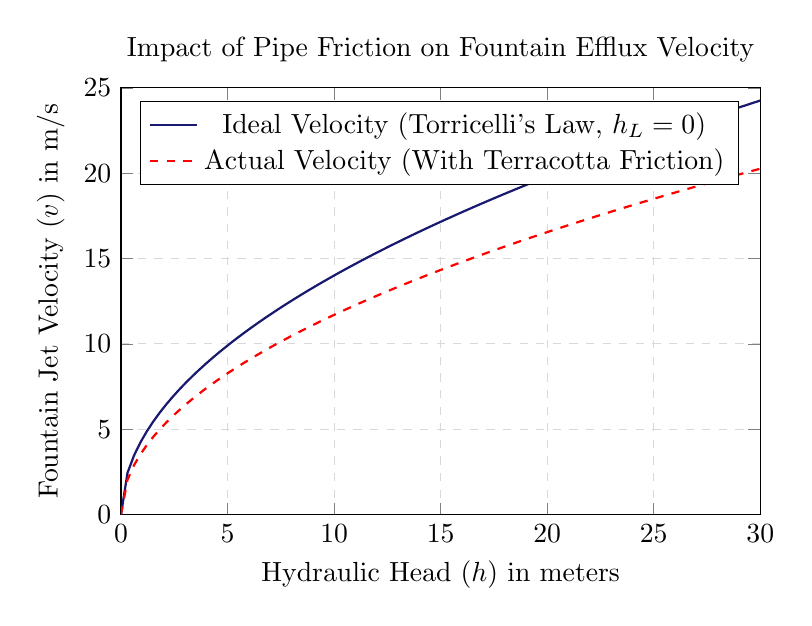
\begin{tikzpicture}
			\begin{axis}[
				width=0.8\textwidth, height=7cm,
				title={Impact of Pipe Friction on Fountain Efflux Velocity},
				xlabel={Hydraulic Head ($h$) in meters}, ylabel={Fountain Jet Velocity ($v$) in m/s},
				xmin=0, xmax=30, ymin=0, ymax=25,
				legend pos=north west, grid=major, grid style={dashed, gray!30},
				]
				% Ideal Velocity v = sqrt(2*g*h) = sqrt(19.62 * h) = 4.429 * sqrt(h)
				\addplot[color=MidnightBlue, thick, domain=0:30, samples=100] {4.429 * sqrt(x)}; 
				\addlegendentry{Ideal Velocity (Torricelli's Law, $h_L=0$)}
				
				% Real Velocity with friction (Assume head loss h_L is roughly 30% of head for long terracotta pipes)
				% v = sqrt(2 * 9.81 * 0.7 * h) = sqrt(13.734 * h) = 3.70 * sqrt(h)
				\addplot[color=red, thick, dashed, domain=0:30, samples=100] {3.70 * sqrt(x)}; 
				\addlegendentry{Actual Velocity (With Terracotta Friction)}
			\end{axis}
		\end{tikzpicture}
		\caption{Comparison of ideal vs. actual fluid velocity. Ancient engineers minimized internal pipe roughness to keep the actual velocity as close to the ideal theoretical curve as possible.}
		\label{fig:friction_velocity}
	\end{figure}
	
	To prevent the terracotta pipes from bursting under this extreme dynamic and turbulent pressure, the pipes were encased in a highly compacted matrix of clay and rubble, which acted as an external compressive reinforcement.
	
	
	
	\subsection{Aerodynamic Anchoring Mechanisms}
	To counteract extreme wind dynamic pressure, engineers carved deep geometric keyholes into the solid bedrock. Massive timber columns were slotted directly into these rock-cut foundations. This interlocking structural matrix transferred horizontal wind loads deep into the immovable rock mass, establishing a state of absolute static equilibrium.
	
	
	\begin{figure}[h]
		\centering
		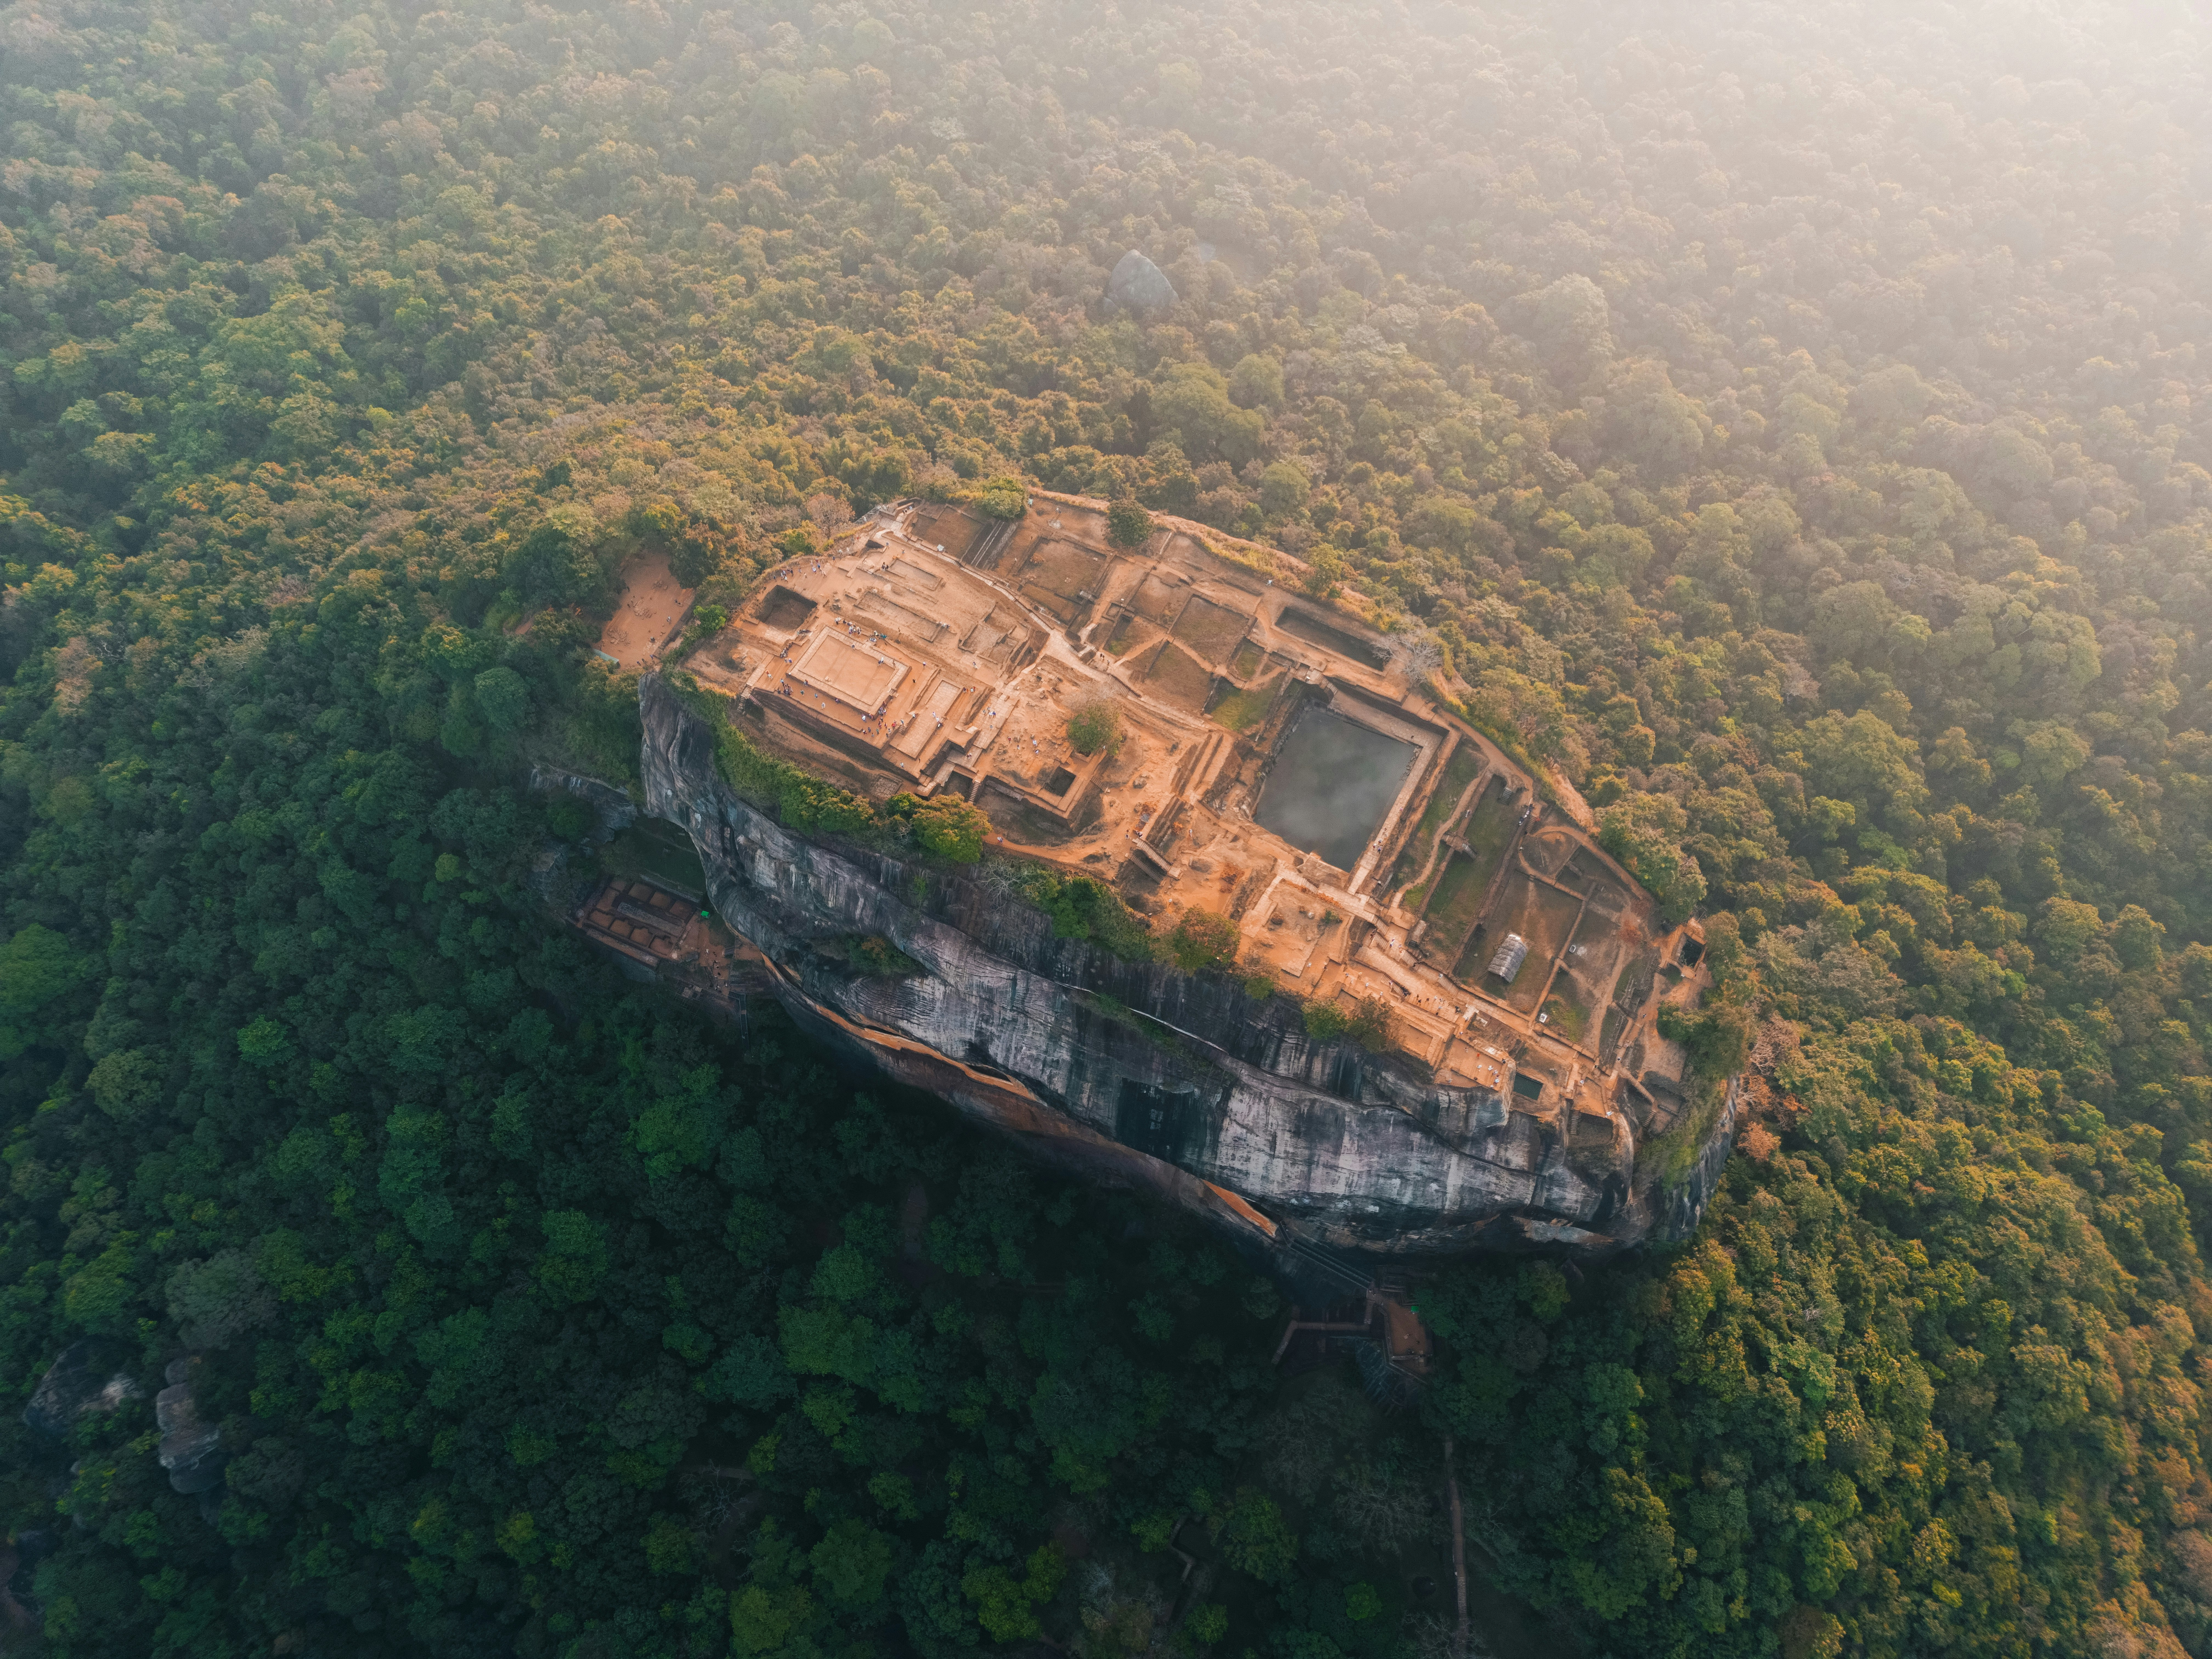
\includegraphics[width=0.8\textwidth]{sigiriya_rock.jpg}
		\caption{The Sigiriya Rock Fortress}
		\label{fig:sigiriya}
	\end{figure}
	
	\begin{figure}[h]
		\centering
		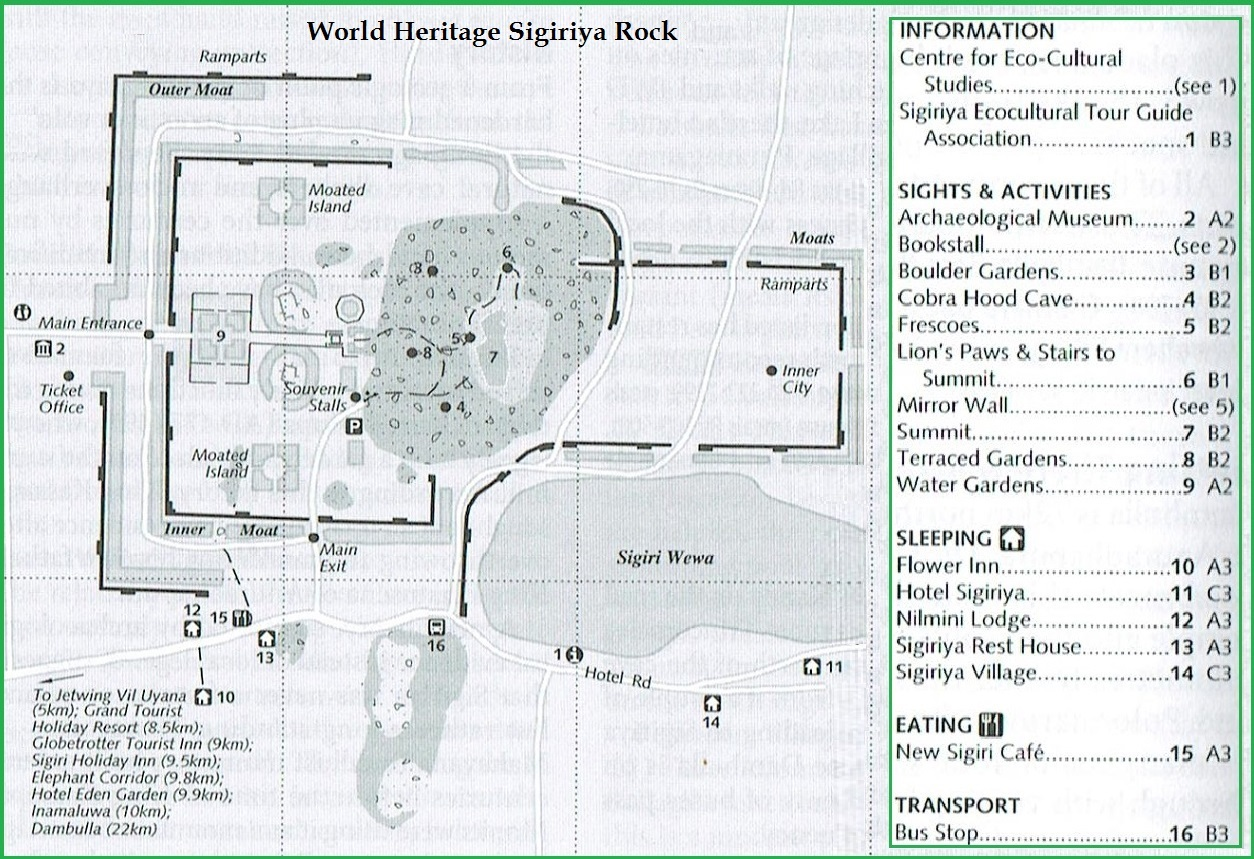
\includegraphics[width=0.8\textwidth]{sigiriya_rock_eng.jpg}
		\caption{Engineering Structures of Sigiriya Rock}
		\label{fig 1:sigiriya}
	\end{figure}
	
	%=========================================
	% CHAPTER 3: JETAVANARAMAYA
	%=========================================
	\chapter{Jetavanaramaya Stupa}
	
	\section{Historical Background}
	Constructed under King Mahasena (273–301 CE), the Jetavanaramaya Stupa is a monumental achievement in ancient masonry. Standing originally at 122 meters, it was the third tallest structure in the ancient world. It required decades of labor and pushed the boundaries of geotechnical engineering far beyond contemporary global standards \cite{wijesuriya1998}.
	
	\section{Construction Materials and Degradation}
	The stupa comprises approximately 93.3 million baked bricks, generating a total volume of $233,000 \, \text{m}^3$. These bricks were bonded using a specialized bio-inorganic mortar containing crushed dolomite limestone, river sand, clay, and organic plant resins \cite{rajapakse2021}. 
	
	Today, the stupa faces severe material degradation. Capillary water absorption draws moisture deep into the porous bricks, dissolving the internal lime mortar matrix. Furthermore, thermal cycling causes micro-cracking, reducing the compressive strength of the outer brick layers.
	
	\begin{figure}[H]
		\centering
		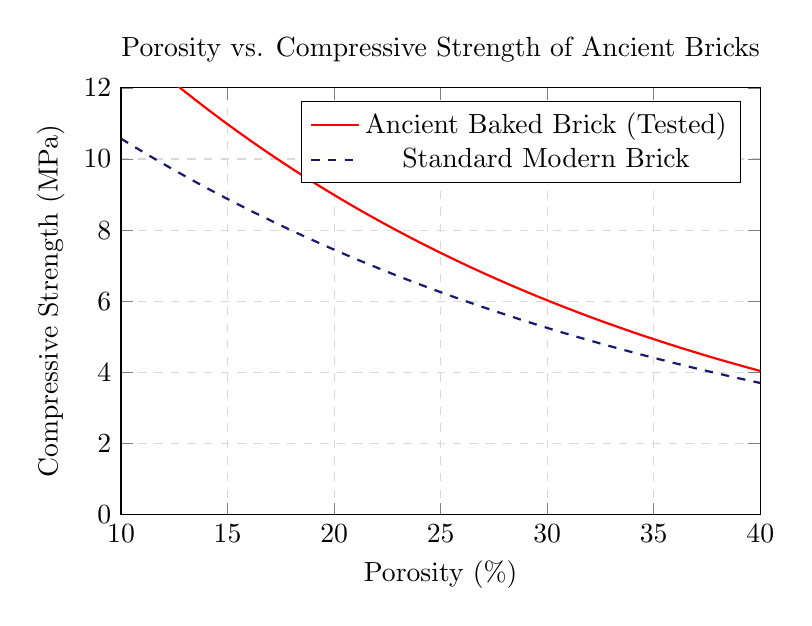
\begin{tikzpicture}
			\begin{axis}[
				width=0.8\textwidth, height=7cm,
				title={Porosity vs. Compressive Strength of Ancient Bricks},
				xlabel={Porosity (\%)}, ylabel={Compressive Strength (MPa)},
				xmin=10, xmax=40, ymin=0, ymax=12,
				legend pos=north east, grid=major, grid style={dashed, gray!30},
				]
				% Empirical relationship: Strength decreases exponentially with porosity
				% S = S_0 * e^(-b*p) where p is porosity fraction. Let S_0 = 20, b = 4.
				\addplot[color=red, thick, domain=10:40, samples=50] {20 * exp(-4 * (x/100))}; 
				\addlegendentry{Ancient Baked Brick (Tested)}
				
				\addplot[color=MidnightBlue, thick, dashed, domain=10:40, samples=50] {15 * exp(-3.5 * (x/100))}; 
				\addlegendentry{Standard Modern Brick}
			\end{axis}
		\end{tikzpicture}
		\caption{Ancient bricks possessed higher porosity to allow the resin-mortar to seep deeply, yet retained remarkably high compressive strength compared to modern equivalents.}
		\label{fig:porosity_strength}
	\end{figure}
	
	\section{Engineering Challenges}
	The total dead mass of the stupa is estimated at $2.5 \times 10^8 \, \text{kg}$, generating a massive base compressive stress of roughly $240 \, \text{kPa}$. Standard tropical sandy-clay soils fail under stresses exceeding $150 \, \text{kPa}$. Preventing catastrophic shear failure of the foundation soil under a circular load was the primary geotechnical hurdle \cite{ratnayake2019}.
	
	\section{Engineering Significance}
	
	\subsection{Terzaghi’s Circular Footing Analysis}
	Ancient engineers solved the shear failure problem using \textit{Dynamic Deep Compaction}. They excavated an 8.5-meter deep trench and used elephants to trample the layered foundation. The ultimate bearing capacity ($q_u$) for a circular foundation is defined by Terzaghi's equation:
	
	\begin{equation}
		q_u = 1.3 c' N_c + q N_q + 0.3 \gamma B N_\gamma
	\end{equation}
	
	Where $c'$ is soil cohesion, $q$ is the surcharge pressure ($\gamma D_f$), $\gamma$ is the unit weight of soil, $B$ is the diameter ($114 \, \text{m}$), and $N_c, N_q, N_\gamma$ are bearing capacity factors. By systematically increasing the depth ($D_f$) to 8.5m and increasing the soil density ($\gamma$) through elephant compaction, the engineers pushed the $q_u$ far beyond the required $240 \, \text{kPa}$, ensuring zero differential settlement.
	
	\begin{table}[H]
		\centering
		\caption{Geotechnical Parameters: Uncompacted vs. Compacted Soil}
		\label{tab:geotech_soil}
		\begin{tabular}{@{}lcc@{}}
			\toprule
			\textbf{Parameter} & \textbf{Natural Tropical Soil} & \textbf{Elephant-Compacted Base} \\ \midrule
			Unit Weight ($\gamma$) & $16 \, \text{kN/m}^3$ & $21 \, \text{kN/m}^3$ \\
			Depth of Foundation ($D_f$) & $1.0 \, \text{m}$ (Standard) & $8.5 \, \text{m}$ (Deep Trench) \\
			Effective Cohesion ($c'$) & $15 \, \text{kPa}$ & $45 \, \text{kPa}$ \\
			Calculated Capacity ($q_u$) & $\approx 180 \, \text{kPa}$ & $\mathbf{> 650 \, \text{kPa}}$ \\ \bottomrule
		\end{tabular}
	\end{table}
	
	\subsection{Hoop Stress Management}
	To counteract outward tensile bursting forces (Hoop stress) at the base of the massive dome, engineers designed three massive retaining rings (\textit{Pesavalalu}). These act as compressive structural bands, neutralizing horizontal tensile forces and safely directing the load vertically downwards.
	
	\begin{figure}[h]
		\centering
		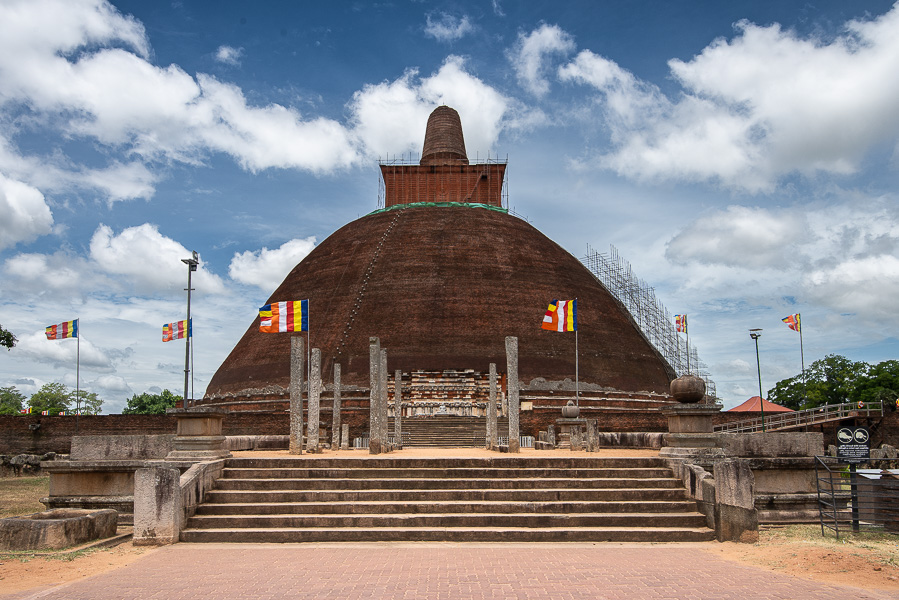
\includegraphics[width=0.8\textwidth]{jetavanaramaya.jpg}
		\caption{Jetavanaramaya Stupa in Anuradhapura}
		\label{fig:jetavanaramaya}
	\end{figure}
	
	\begin{figure}[h]
		\centering
		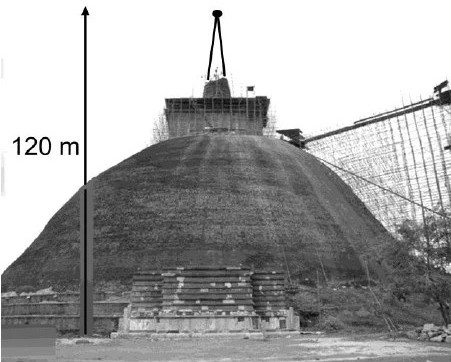
\includegraphics[width=0.8\textwidth]{jetavanaramaya_eng.jpg}
		\caption{Engineering Structures of Jetavanaramaya Stupa}
		\label{fig 1:jetavanaramaya}
	\end{figure}
	
	%=========================================
	% CHAPTER 4: JAYA GANGA
	%=========================================
	\chapter{Jaya Ganga (Yoda Ela)}
	
	\section{Historical Background}
	Built in the 5th century under King Dhatusena, the 87-kilometer Jaya Ganga was the central artery of Sri Lanka's ancient agricultural revolution. It carried water from the colossal Kalawewa reservoir to the Tissa Wewa, supplying irrigation to hundreds of cascading village tanks along its route \cite{jayawardena2017}.
	
	\section{Construction Materials and Degradation}
	The embankments were constructed using highly compacted laterite soils and clay. The sluice gates (\textit{Bisokotuwa}), which regulated water pressure entering the canal, were constructed using finely dressed crystalline limestone blocks. Today, unauthorized deforestation, changing climate patterns, and agricultural encroachment cause severe scouring (erosion) and siltation, threatening the canal's meticulously engineered flow regime \cite{senanayake2021}.
	
	\section{Engineering Challenges}
	The canal had to traverse undulating terrain without mechanical pumps. Releasing highly pressurized water directly from the deep Kalawewa reservoir into an earthen canal would instantly destroy the banks. Therefore, engineers had to invent a mechanism to dissipate immense hydrostatic pressure before the water entered the canal. Furthermore, the canal's gradient had to be flawlessly balanced to prevent both erosion and siltation.
	
	\section{Engineering Significance}
	
	\subsection{The Bisokotuwa (Ancient Surge Chamber)}
	Before water entered the Jaya Ganga, it passed through the \textit{Bisokotuwa} (Valve Pit). As water exits a deep reservoir under high pressure ($P = \rho g h$), its kinetic energy is enormous. The Bisokotuwa acted as an expansion chamber. As water entered this wider chamber, its velocity dropped dramatically according to the principle of continuity ($A_1V_1 = A_2V_2$), safely dissipating the destructive kinetic energy before it flowed into the fragile earthen canal.
	
	\subsection{Manning's Equation and Canal Gradient}
	The Jaya Ganga features an extraordinarily microscopic gradient of roughly 0.0001 (a drop of merely 10 to 20 cm per kilometer). The flow dynamics are perfectly modeled by Manning's Equation:
	
	\begin{equation}
		V = \frac{1}{n} R^{2/3} S^{1/2}
	\end{equation}
	
	Where $V$ is flow velocity, $n$ is the roughness coefficient (approx. 0.025 for earthen channels), $R$ is the hydraulic radius, and $S$ is the channel slope. 
	
	\begin{figure}[H]
		\centering
		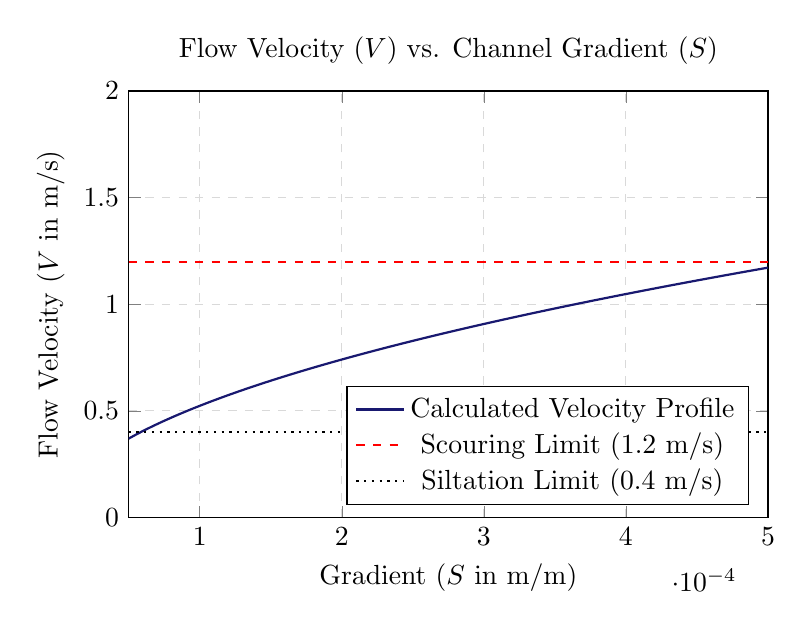
\begin{tikzpicture}
			\begin{axis}[
				width=0.8\textwidth, height=7cm,
				title={Flow Velocity ($V$) vs. Channel Gradient ($S$)},
				xlabel={Gradient ($S$ in m/m)}, ylabel={Flow Velocity ($V$ in m/s)},
				xmin=0.00005, xmax=0.0005, ymin=0, ymax=2,
				legend pos=south east, grid=major, grid style={dashed, gray!30},
				]
				% Assume Hydraulic Radius R = 1.5m. R^(2/3) = 1.31. n = 0.025
				% V = (1/0.025) * 1.31 * sqrt(S) = 52.4 * sqrt(S)
				\addplot[color=MidnightBlue, thick, domain=0.00005:0.0005, samples=100] {52.4 * sqrt(x)}; 
				\addlegendentry{Calculated Velocity Profile}
				
				\addplot[color=red, thick, dashed, domain=0.00005:0.0005] {1.2 + 0*x};
				\addlegendentry{Scouring Limit (1.2 m/s)}
				
				\addplot[color=black, thick, dotted, domain=0.00005:0.0005] {0.4 + 0*x};
				\addlegendentry{Siltation Limit (0.4 m/s)}
			\end{axis}
		\end{tikzpicture}
		\caption{Manning's Velocity model. The chosen gradient of 0.0001 (0.01\%) perfectly maintains the velocity between the siltation limit (too slow) and the scouring limit (too fast).}
		\label{fig:manning_velocity}
	\end{figure}
	
	Ancient engineers utilized water-leveling instruments (\textit{Diya Katta}) to trace natural elevation contours, creating a \textit{Single-Bank Contour Canal} that actively intercepted surface runoff from higher ground.
	
	\begin{figure}[h]
		\centering
		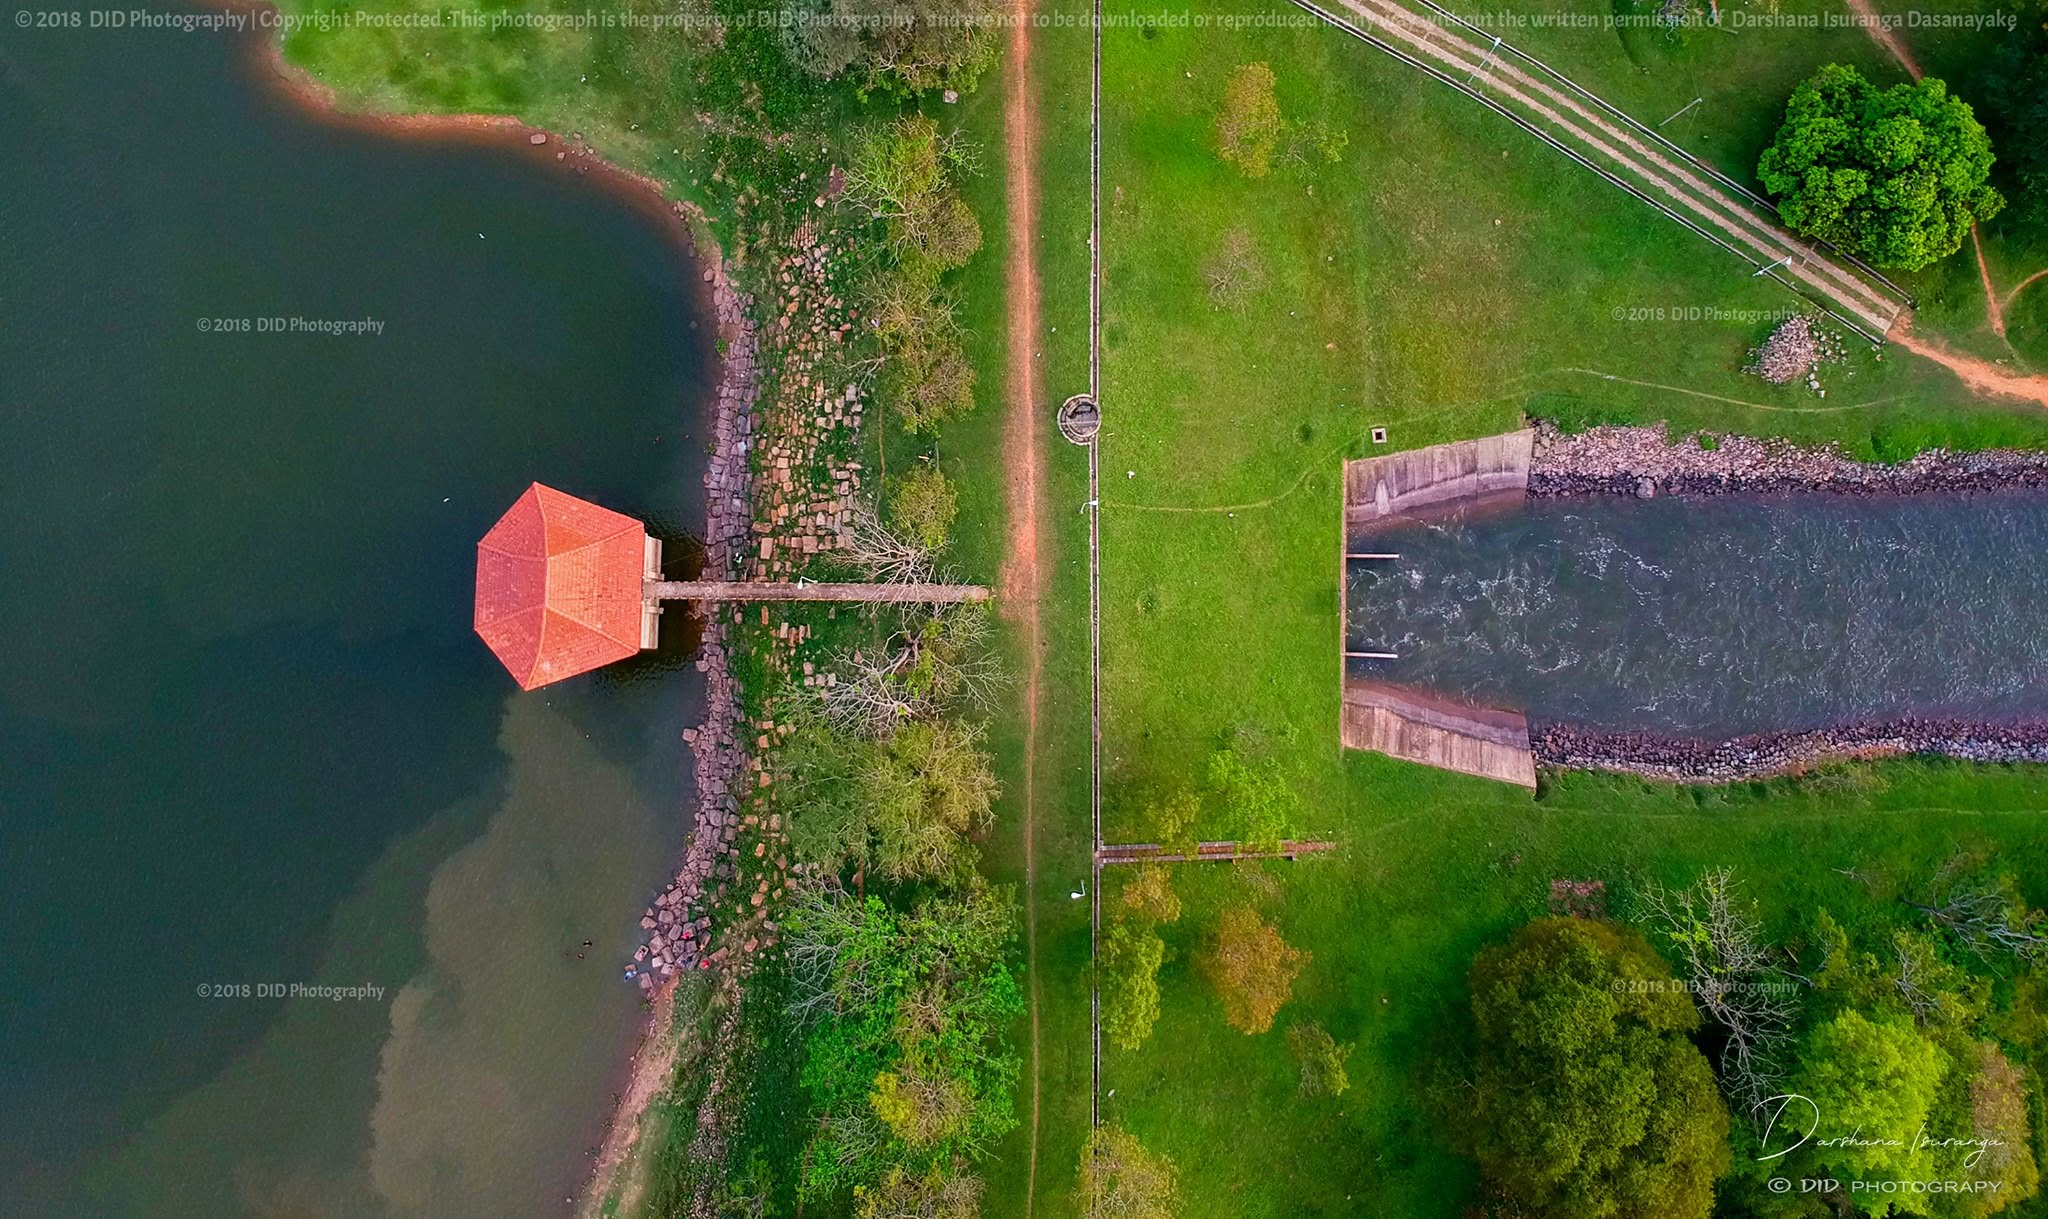
\includegraphics[width=0.8\textwidth]{Jaya_Ganga.jpg}
		\caption{The Flow of Jaya Ganga (Yoda Ela)}
		\label{fig:jayaganga}
	\end{figure}
	
	\begin{figure}[h]
		\centering
		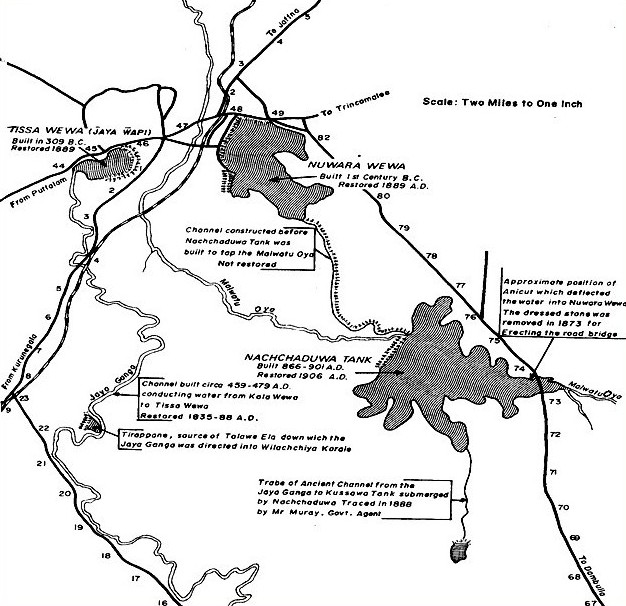
\includegraphics[width=0.8\textwidth]{Jaya_Ganga_eng.jpg}
		\caption{Engineering Structures of Jaya Ganga (Yoda Ela)}
		\label{fig 1:jayaganga}
	\end{figure}
	
	
	%=========================================
	% CHAPTER 5: NINE ARCHES BRIDGE
	%=========================================
	\chapter{Nine Arches Bridge}
	
	\section{Historical Background}
	Completed in 1921, the Nine Arches Bridge is an iconic railway viaduct spanning 91 meters across a deep gorge. Engineered by P.K. Appuhami and D.J. Wimalasurendra during British colonial rule, it connected the lucrative highland tea plantations with the Colombo port \cite{perera2014}.
	
	\section{Construction Materials and Degradation}
	Due to World War I material shortages, the bridge was constructed with \textbf{zero tensile steel reinforcement}, utilizing only solid rock, brick, and cement mortar. Today, after a century of heavy locomotive vibrations and tropical weathering, the mortar is exhibiting signs of structural fatigue, efflorescence, and microscopic shear cracking \cite{karunaratne2015}.
	
	\begin{table}[H]
		\centering
		\caption{Locomotive Live Load Evolution on the Nine Arches Bridge}
		\label{tab:train_loads}
		\begin{tabular}{@{}lcc@{}}
			\toprule
			\textbf{Era / Locomotive Type} & \textbf{Average Axle Load} & \textbf{Dynamic Impact Factor} \\ \midrule
			1920s: Steam Locomotives & 12 - 14 Tons & High (Pounding effect) \\
			1960s: Early Diesel-Electric & 15 - 16 Tons & Medium \\
			2020s: Class M6/M9 Locomotives & 16.5 - 18 Tons & High (Increased speed) \\ \bottomrule
		\end{tabular}
	\end{table}
	
	\section{Engineering Challenges}
	Designing a structure capable of supporting extreme dynamic locomotive loads using only brittle masonry (which easily snaps under bending stress) required flawless mathematical precision in geometric load-paths. Furthermore, the valley floor was a boggy quagmire, requiring deep bedrock excavation for the piers.
	\newpage
	\section{Engineering Significance}
	
	\subsection{Voussoir Arch Statics and Horizontal Thrust}
	Without steel, the bridge relies on \textit{Voussoir Arches}. The parabolic geometry resolves vertical loads purely as compressive forces. A critical calculation in arch design is the Horizontal Thrust ($H$) at the abutments/piers, given by:
	
	\begin{equation}
		H = \frac{w L^2}{8 f}
	\end{equation}
	
	Where $w$ is the uniform load per unit length, $L$ is the span of the arch, and $f$ is the rise (height) of the arch. By optimizing the rise ($f$), engineers minimized the horizontal thrust, allowing the piers to remain stable under massive loads without toppling.
	
	\begin{figure}[H]
		\centering
		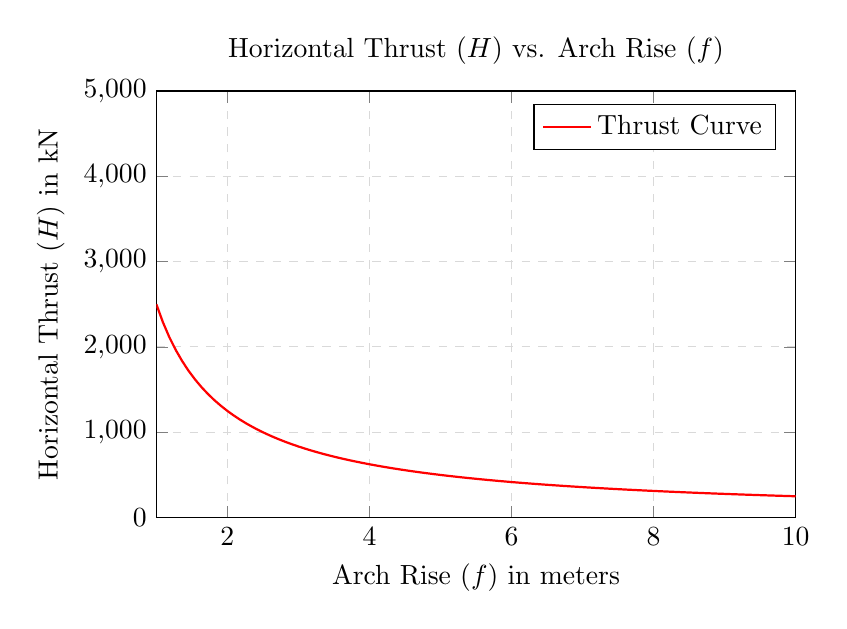
\begin{tikzpicture}
			\begin{axis}[
				width=0.8\textwidth, height=7cm,
				title={Horizontal Thrust ($H$) vs. Arch Rise ($f$)},
				xlabel={Arch Rise ($f$) in meters}, ylabel={Horizontal Thrust ($H$) in kN},
				xmin=1, xmax=10, ymin=0, ymax=5000,
				legend pos=north east, grid=major, grid style={dashed, gray!30},
				]
				% Assume w = 200 kN/m, L = 10m. H = (200 * 100) / (8 * f) = 2500 / f
				\addplot[color=red, thick, domain=1:10, samples=100] {2500 / x}; 
				\addlegendentry{Thrust Curve}
			\end{axis}
		\end{tikzpicture}
		\caption{As the arch rise ($f$) increases, the horizontal thrust pushing the piers apart decreases dramatically. The Nine Arches Bridge utilizes deep parabolic curves to minimize this destructive thrust.}
		\label{fig:horizontal_thrust}
	\end{figure}
	
	\subsection{Dynamic Resonance Dampening}
	The composite masonry acts as a natural dampener for dynamic resonance caused by trains. The dampening of vibrations is modeled as a damped harmonic oscillator:
	\begin{equation}
		x(t) = X_0 e^{-\zeta \omega_n t} \cos(\omega_d t)
	\end{equation}
	Where $\zeta$ is the damping ratio of the masonry matrix. Unlike steel, which has a low damping ratio and vibrates extensively, the millions of microscopic interfaces within the brick-and-mortar matrix absorb kinetic energy rapidly, preventing catastrophic structural fatigue.
	
	\begin{figure}[h]
		\centering
		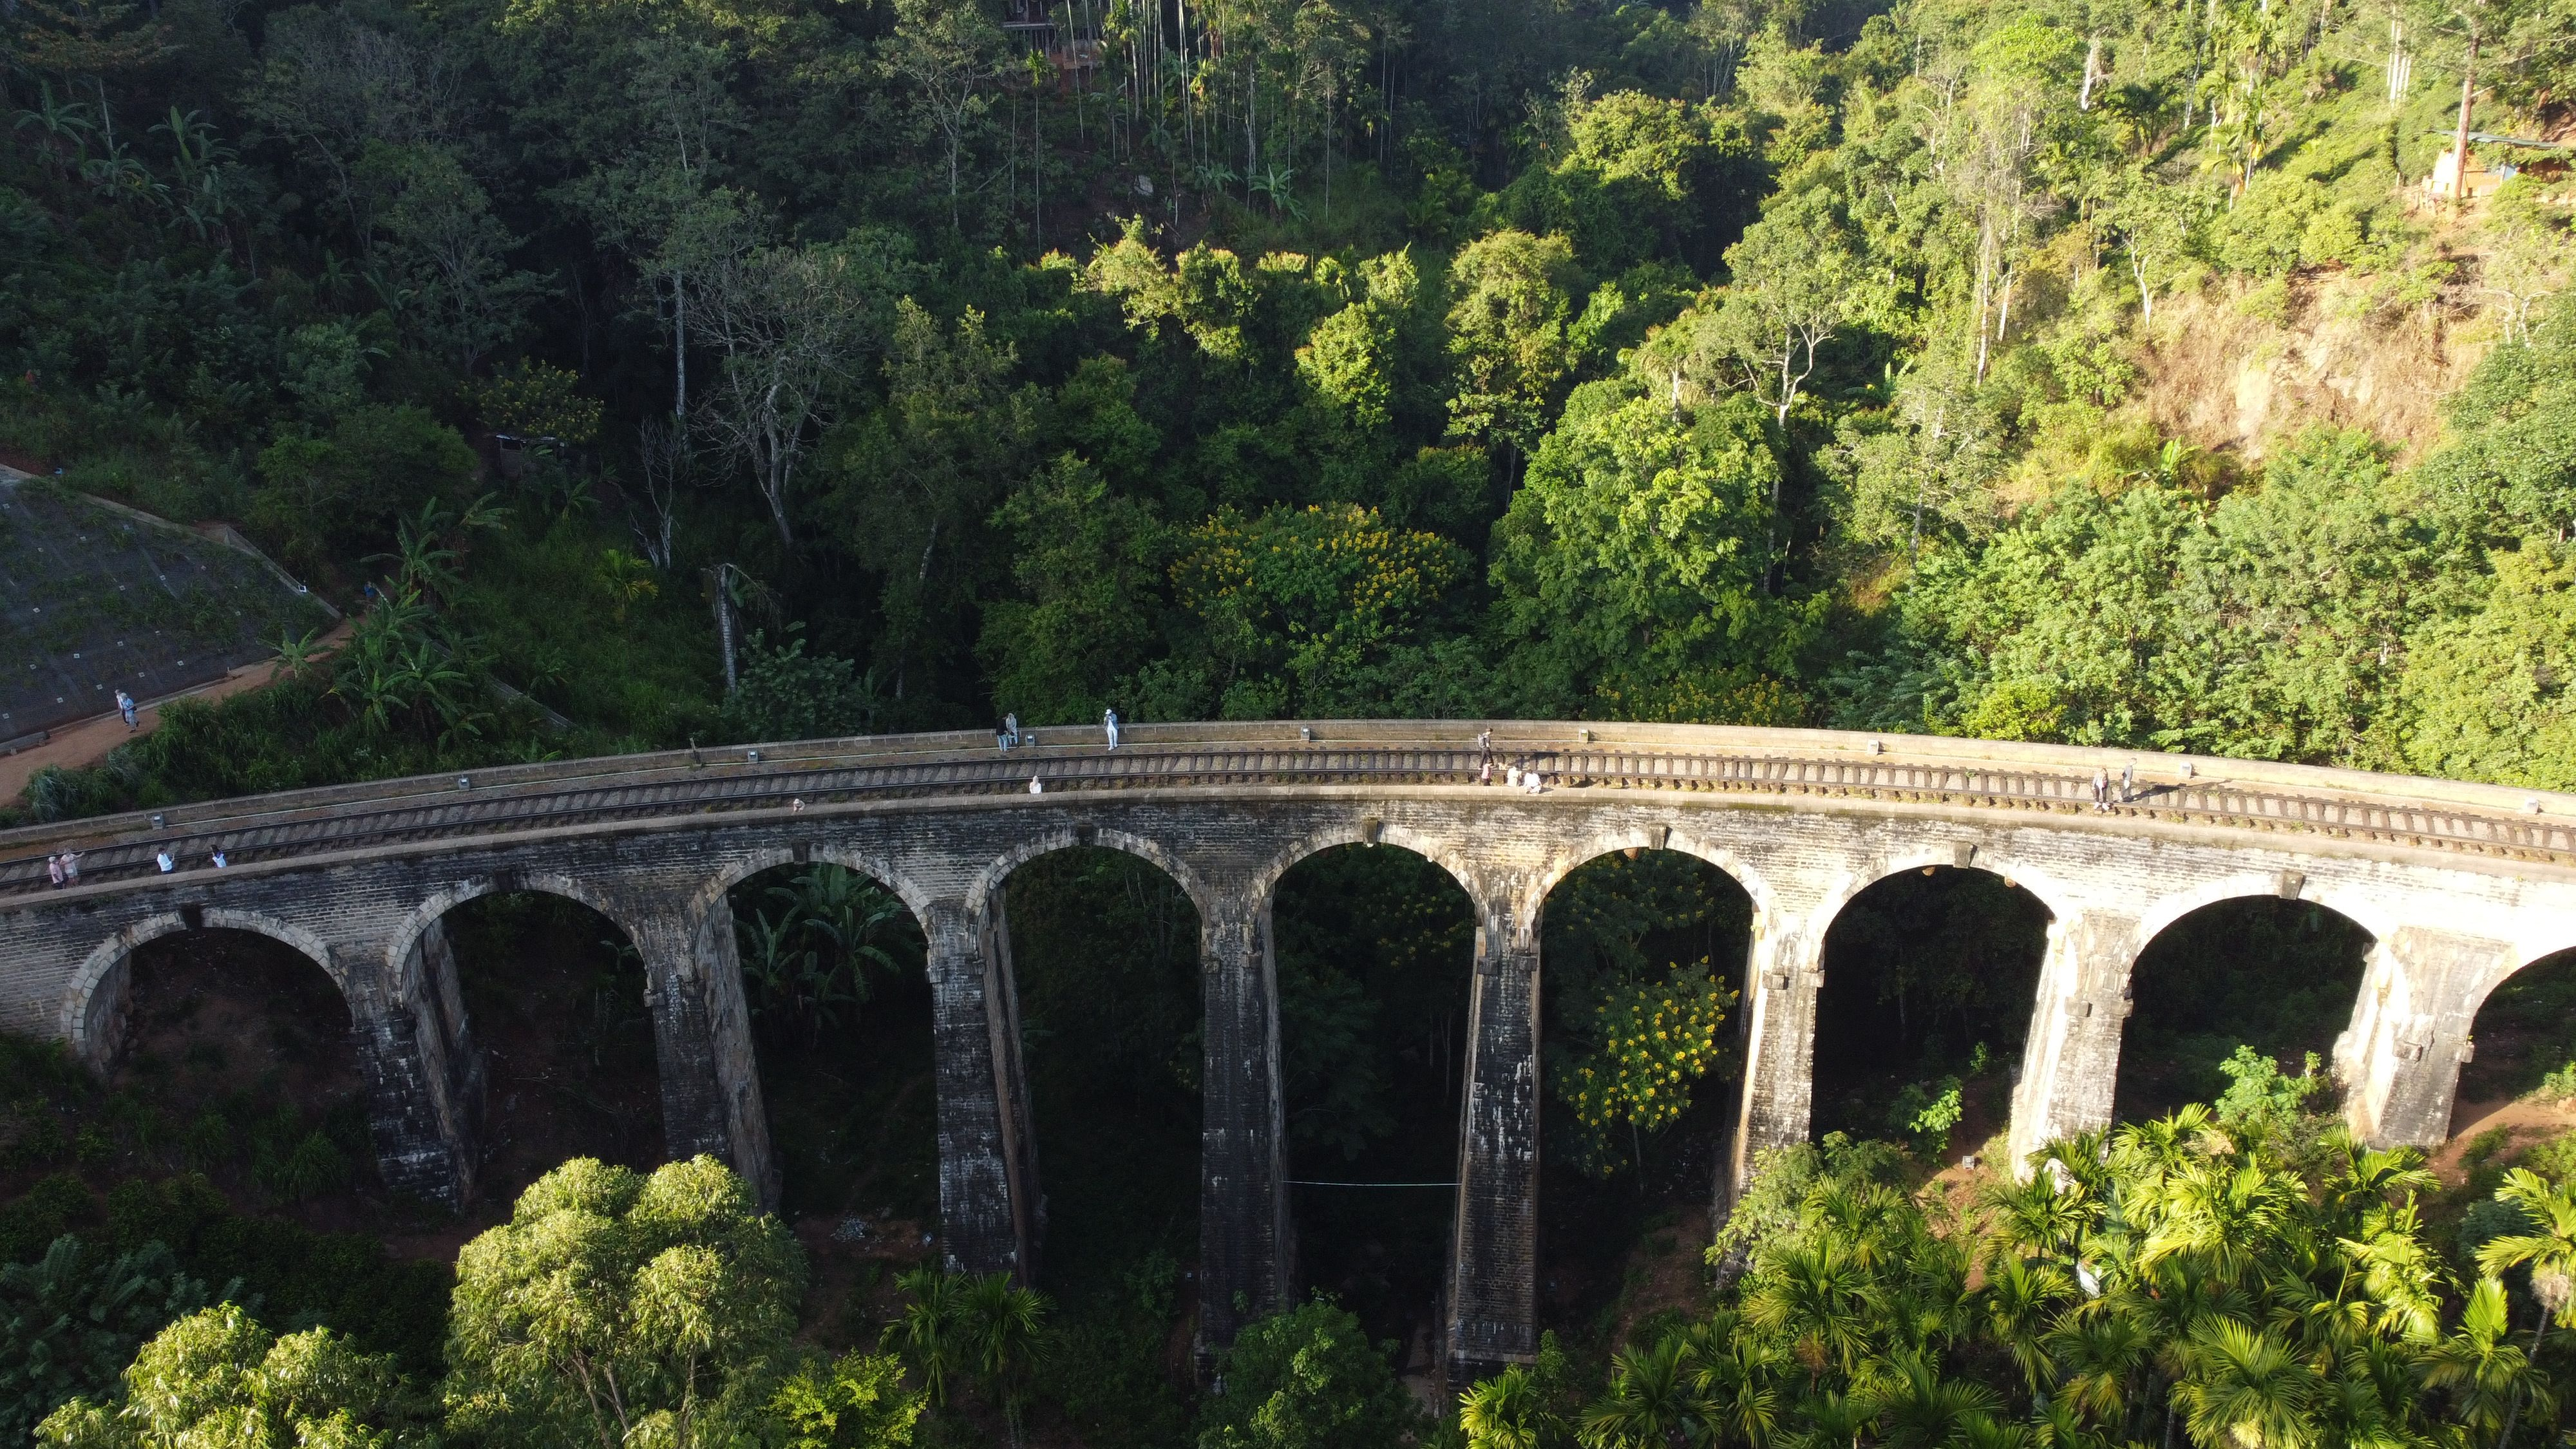
\includegraphics[width=0.8\textwidth]{Nine_Arches_Bridge.jpg}
		\caption{The Nine Arches Bridge in Ella}
		\label{fig:ninearches}
	\end{figure}
	
	\begin{figure}[h]
		\centering
		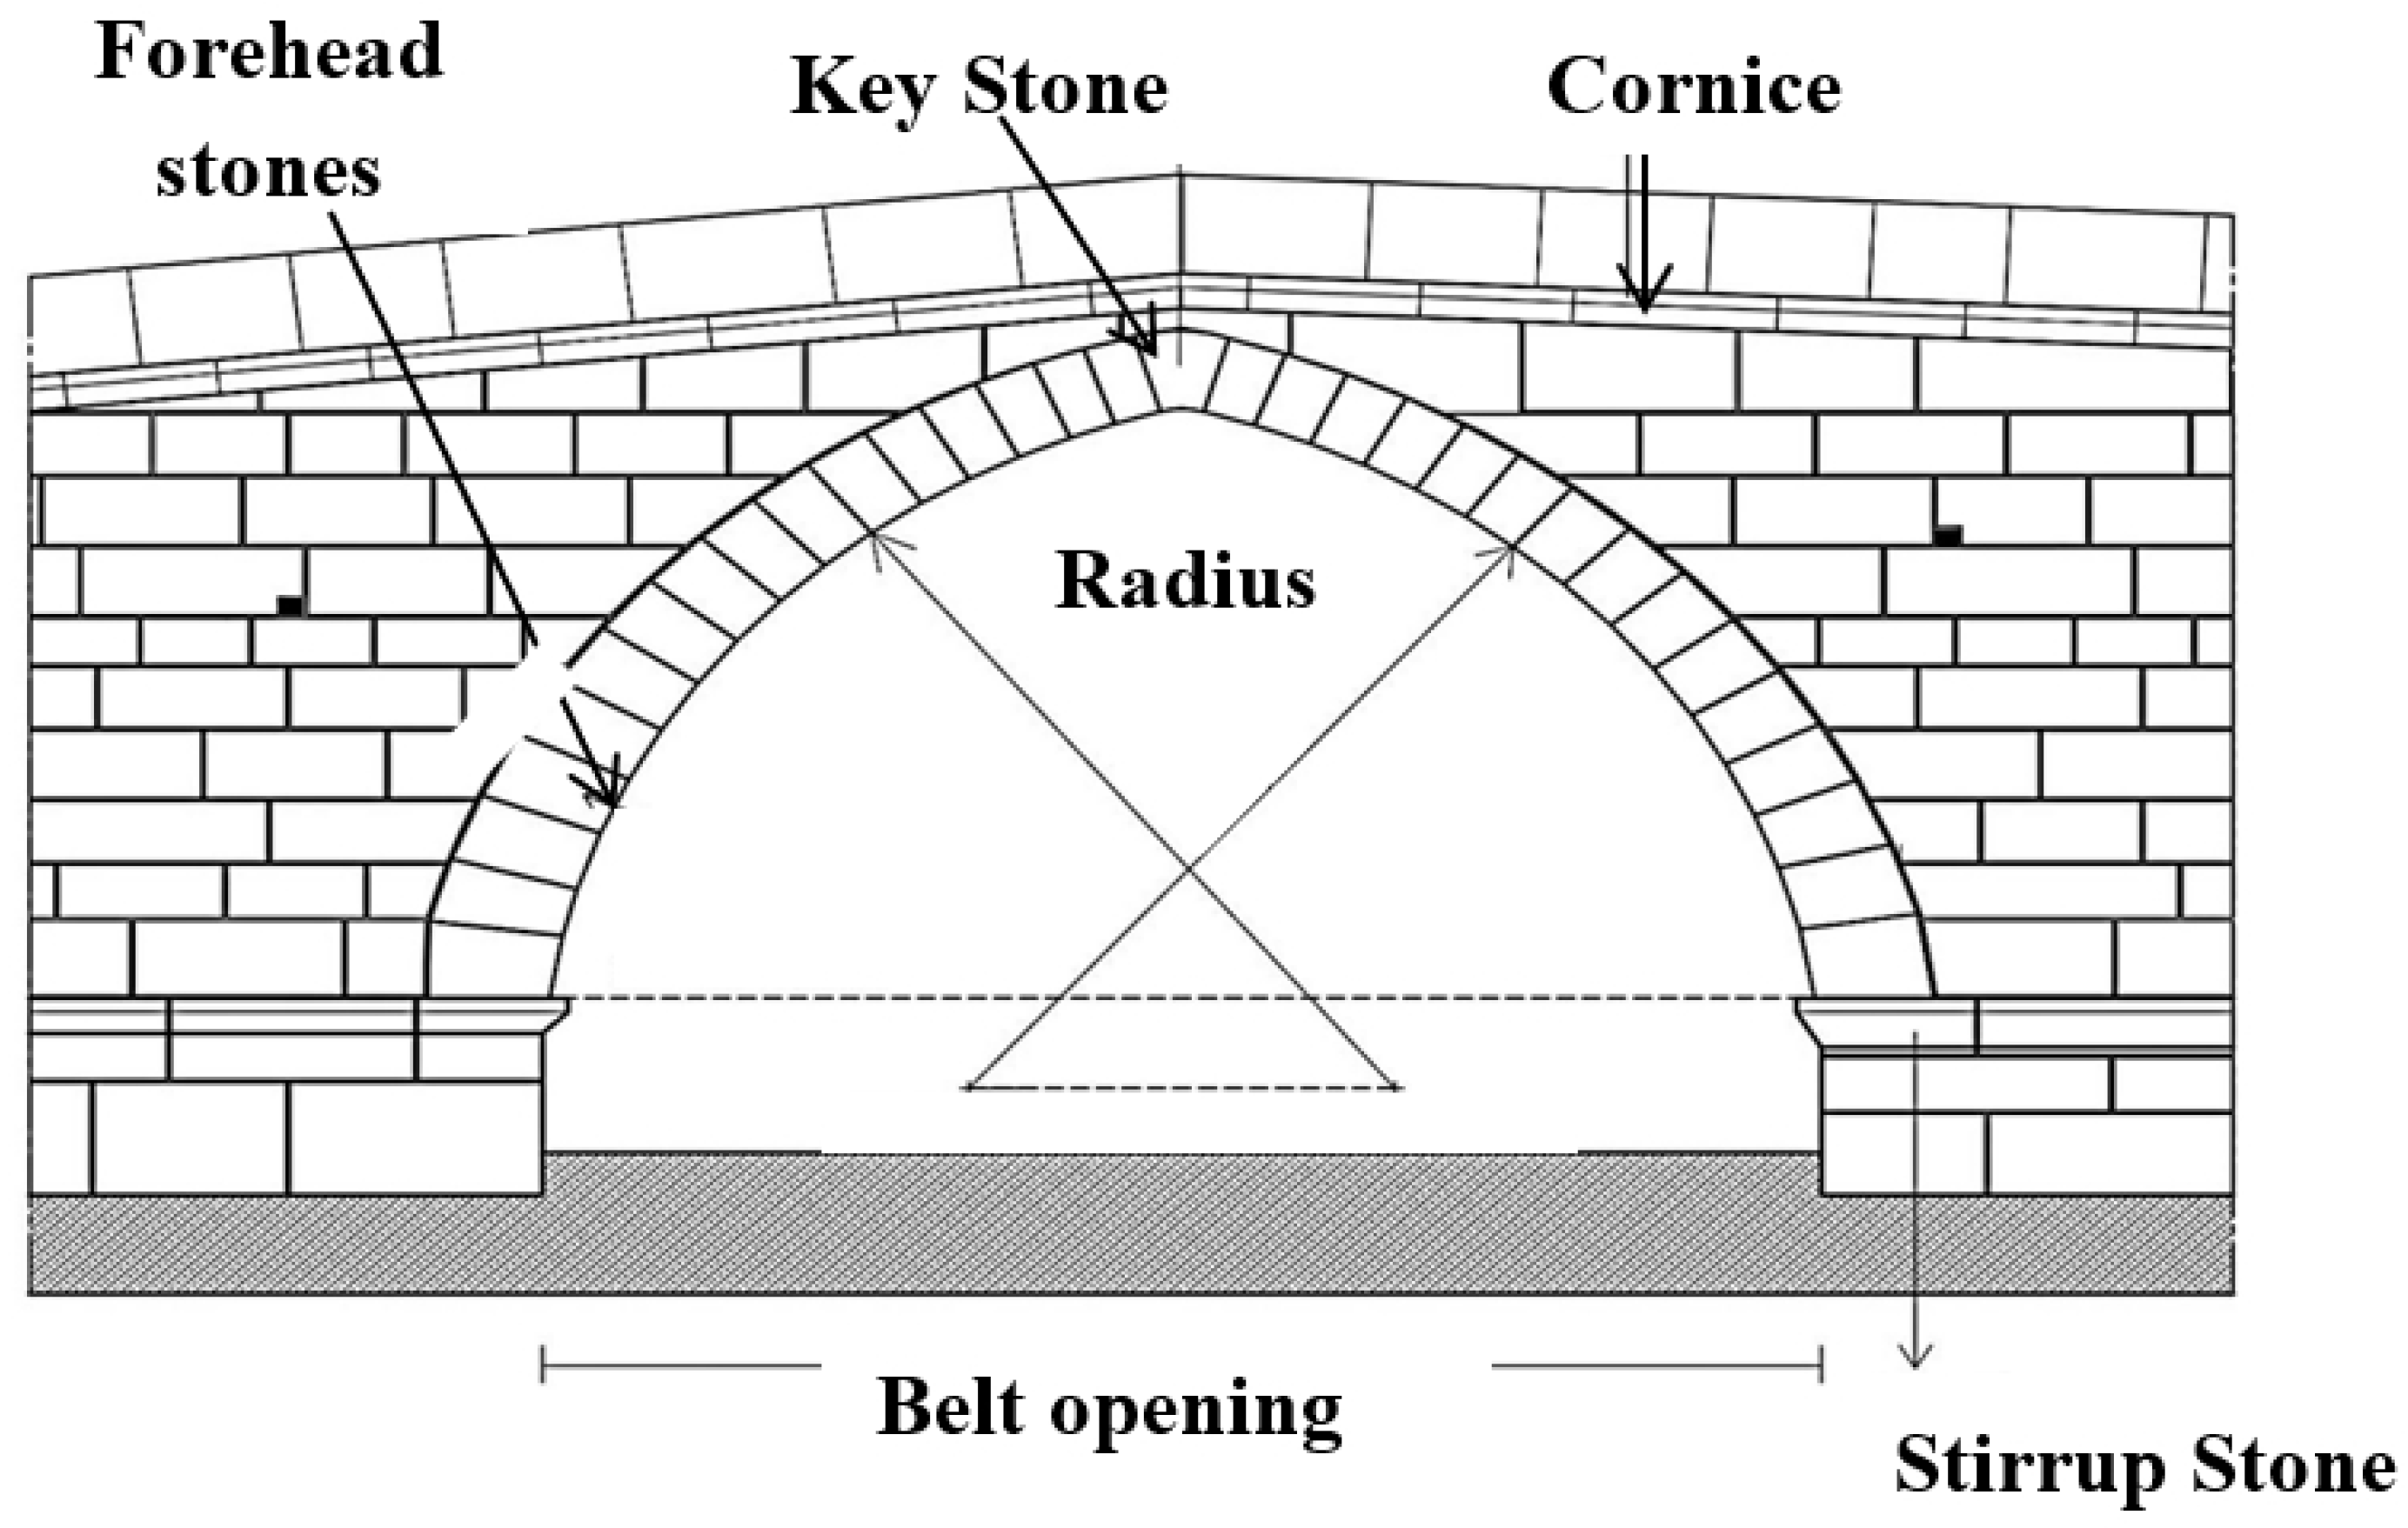
\includegraphics[width=0.8\textwidth]{Nine_Arches_Bridge_eng.jpg}
		\caption{Engineering Structures of The Nine Arches Bridge}
		\label{fig 1:ninearches}
	\end{figure}
	
	
	%=========================================
	% CHAPTER 6: VICTORIA DAM
	%=========================================
	\chapter{Victoria Dam}
	
	\section{Historical Background}
	Completed in 1985, the Victoria Dam is the tallest dam in Sri Lanka (122m). Situated in a deep gorge on the Mahaweli River, its primary objectives are large-scale hydroelectric power (210 MW) and regulating irrigation \cite{halcrow1985}.
	
	\section{Construction Materials and Degradation}
	Constructed from mass concrete using low-heat Portland cement. Currently, the massive impoundment induces localized stress in the bedrock (Reservoir-Induced Seismicity), while upstream deforestation accelerates severe reservoir siltation. Additionally, the concrete spillways face cavitation and hydro-abrasion from high-velocity water \cite{dias2018}.
	
	\section{Engineering Challenges}
	The impounded water (722 million cubic meters) creates astronomical hydrostatic pressure. A standard gravity dam would have required an uneconomical volume of concrete. Additionally, controlling the exothermic heat (heat of hydration) during millions of cubic meters of concrete pouring was a massive thermodynamic challenge \cite{fernando2022}.
	
	\section{Engineering Significance}
	
	\subsection{Integration of Hydrostatic Force}
	The pressure exerted by water at any depth $y$ is $P = \rho g y$. The total hydrostatic force ($F$) on the face of the dam is found by integrating this pressure over the depth ($H$) and width ($W$):
	
	\begin{equation}
		F = \int_{0}^{H} (\rho g y) W \, dy = \frac{1}{2} \rho g W H^2
	\end{equation}
	
	Because the force increases with the \textit{square} of the depth ($H^2$), the base of the dam must withstand extreme loads. 
	
	\begin{figure}[H]
		\centering
		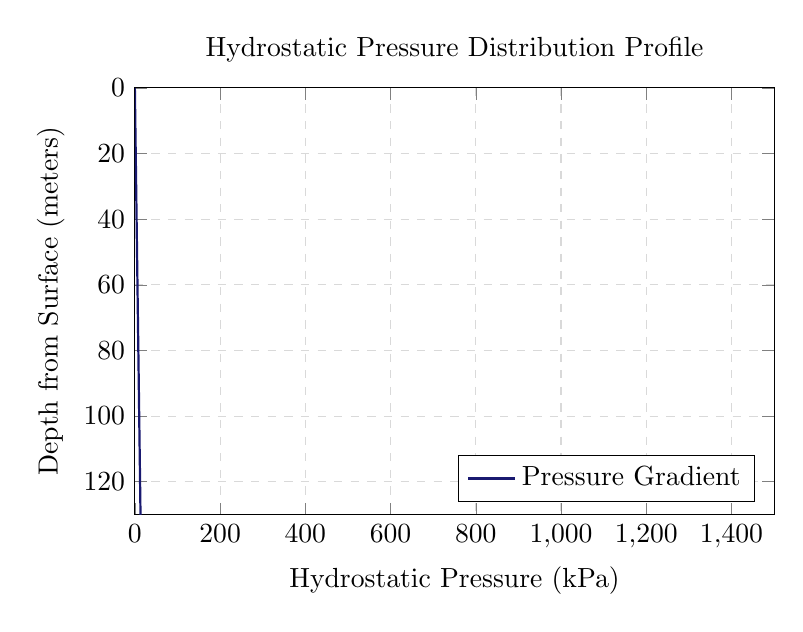
\begin{tikzpicture}
			\begin{axis}[
				width=0.8\textwidth, height=7cm,
				title={Hydrostatic Pressure Distribution Profile},
				xlabel={Hydrostatic Pressure (kPa)}, ylabel={Depth from Surface (meters)},
				xmin=0, xmax=1500, ymin=0, ymax=130,
				y dir=reverse, % Depth goes downwards
				legend pos=south east, grid=major, grid style={dashed, gray!30},
				]
				% P = rho * g * h = 1000 * 9.81 * h / 1000 (to get kPa) = 9.81 * h
				\addplot[color=MidnightBlue, thick, domain=0:122, samples=50] {9.81 * x}; 
				\addlegendentry{Pressure Gradient}
			\end{axis}
		\end{tikzpicture}
		\caption{Hydrostatic pressure increases linearly with depth, reaching over 1,100 kPa at the base of the Victoria Dam.}
		\label{fig:hydrostatic_pressure}
	\end{figure}
	
	The Victoria Dam utilizes a \textit{Double Curvature Arch} design to handle this force. It is curved both horizontally and vertically, transferring the massive hydraulic thrust outwards into the solid rock abutments rather than relying purely on mass.
	
	\subsection{Thermodynamic Mass Concrete Management}
	To prevent thermal cracking during construction, engineers chilled the aggregates and water prior to mixing. This thermodynamic control ensured the peak exothermic temperature remained safely below the critical cracking threshold, allowing for monolithic structural integrity.
	
	\begin{figure}[h]
		\centering
		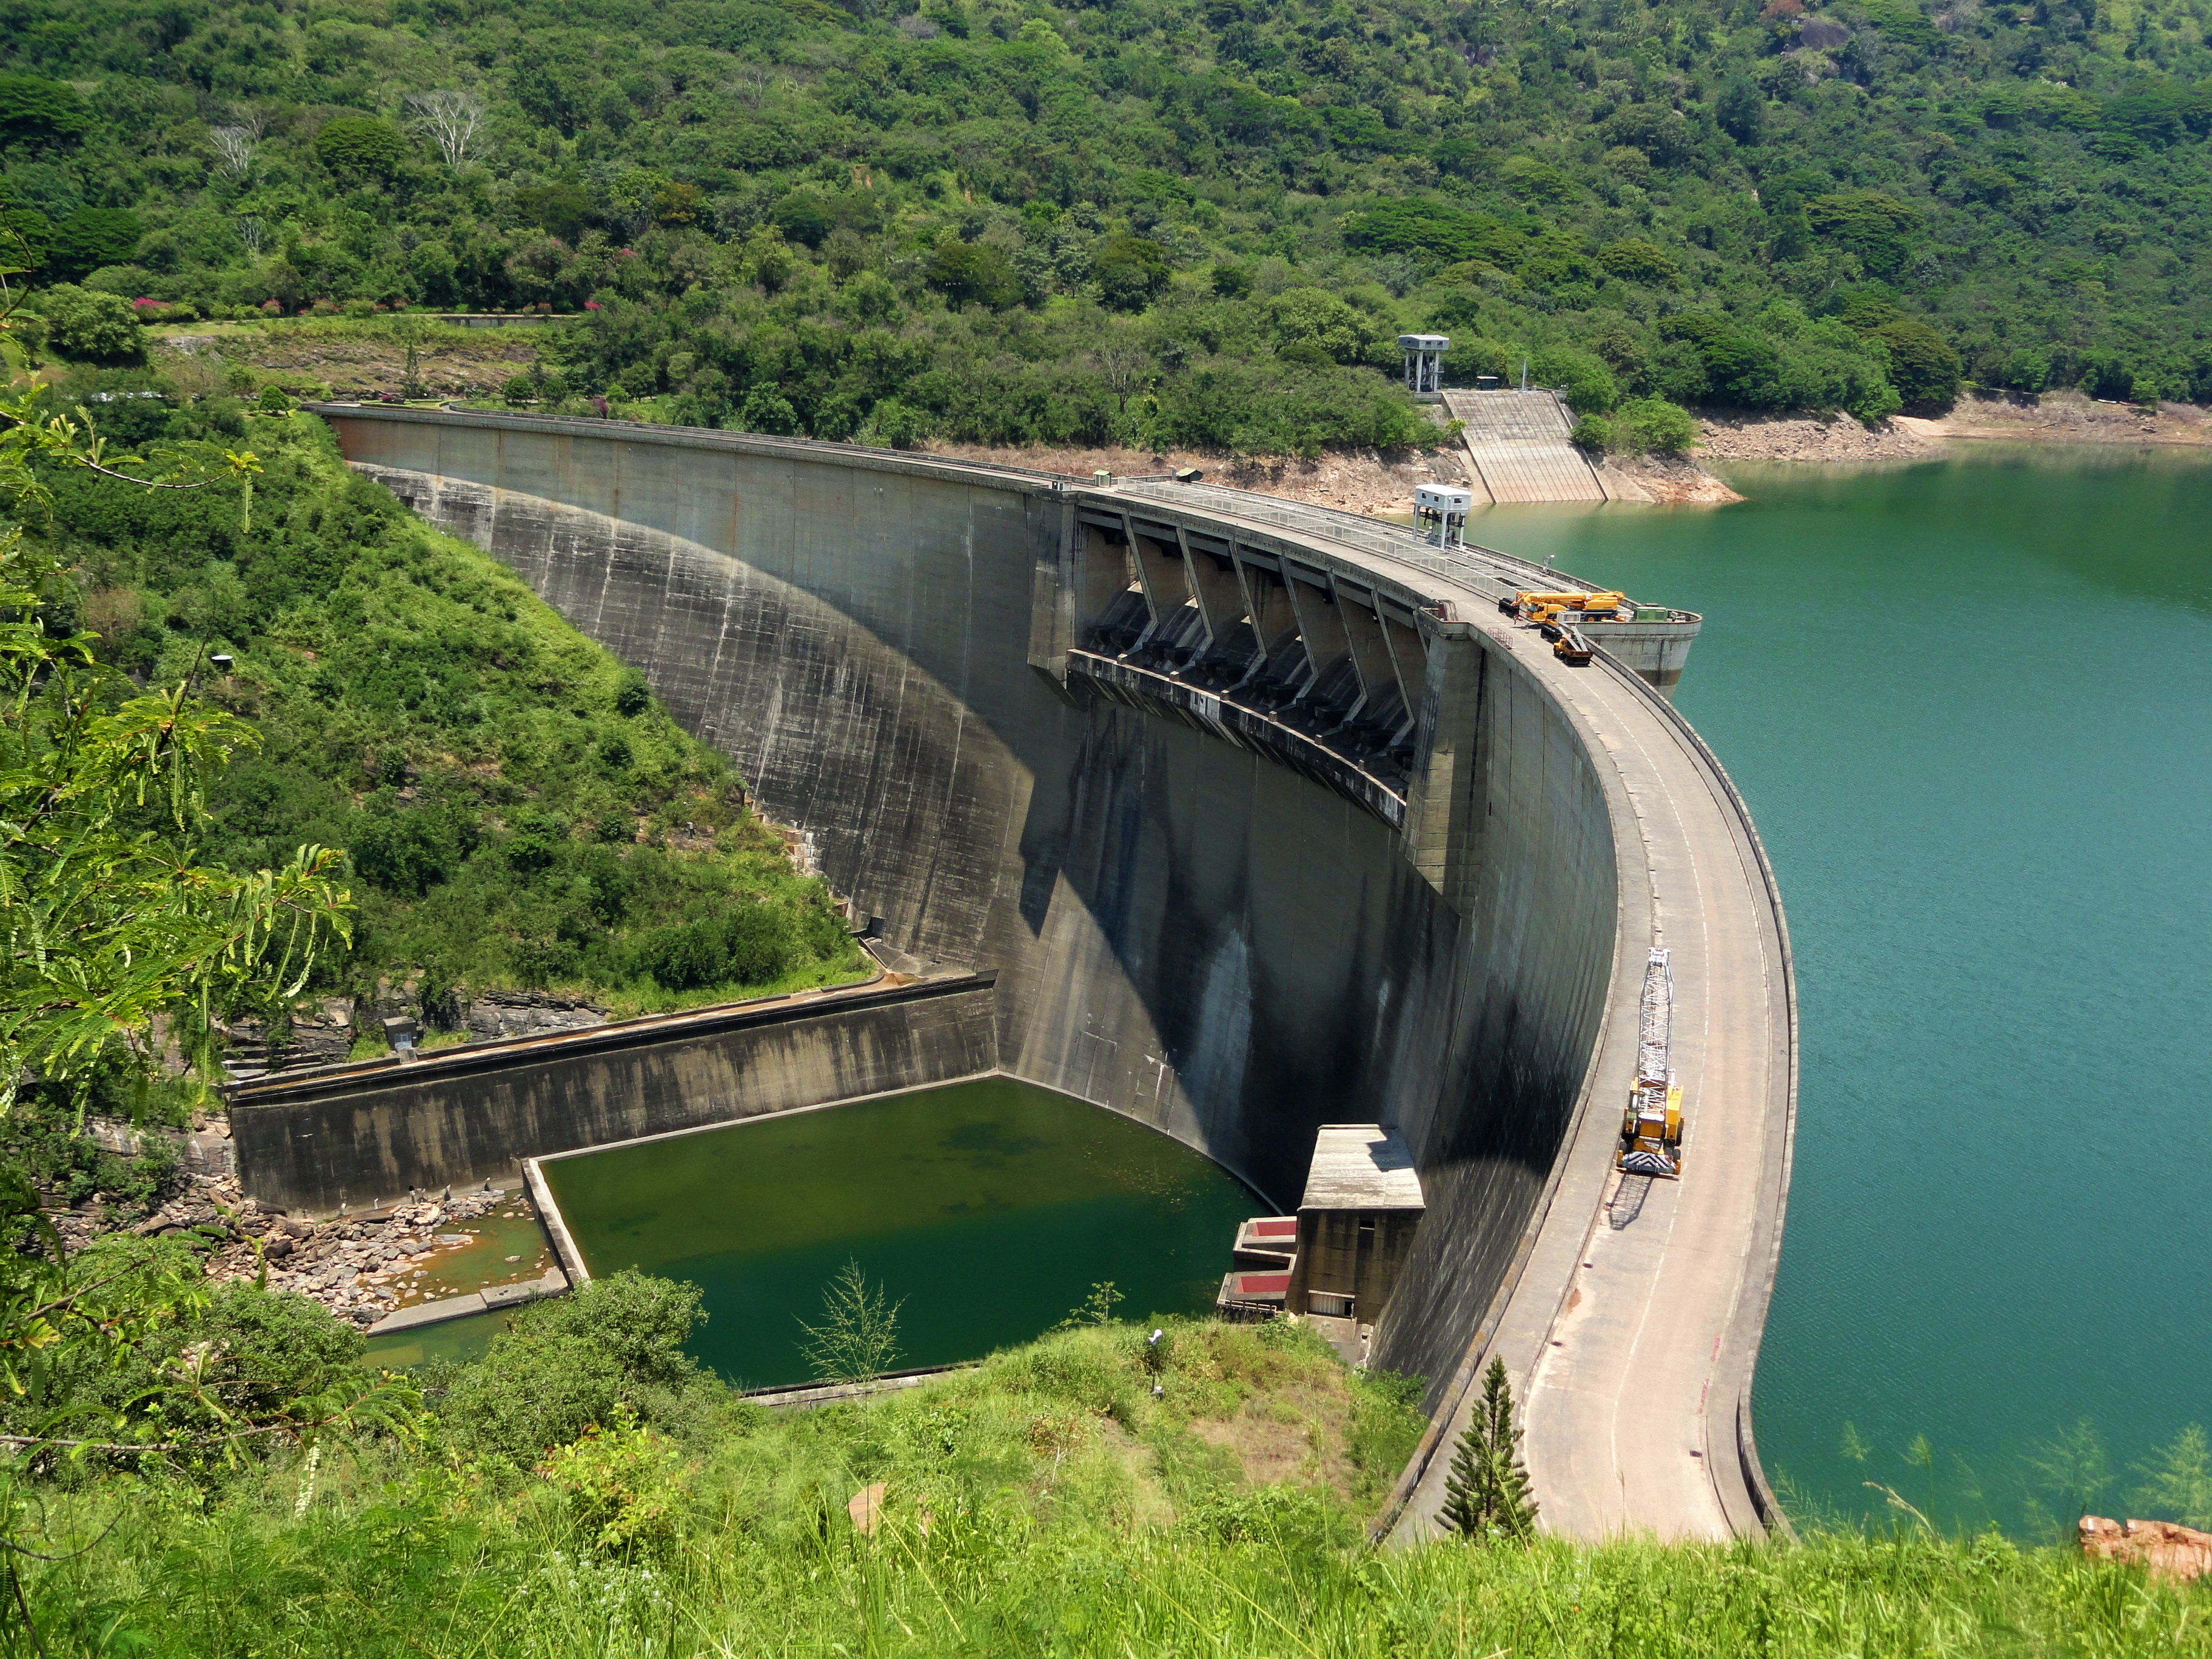
\includegraphics[width=0.8\textwidth]{Victoria_Dam.jpg}
		\caption{The Victoria Dam Double Curvature Arch}
		\label{fig:victoriadam}
	\end{figure}
	
	\begin{figure}[h]
		\centering
		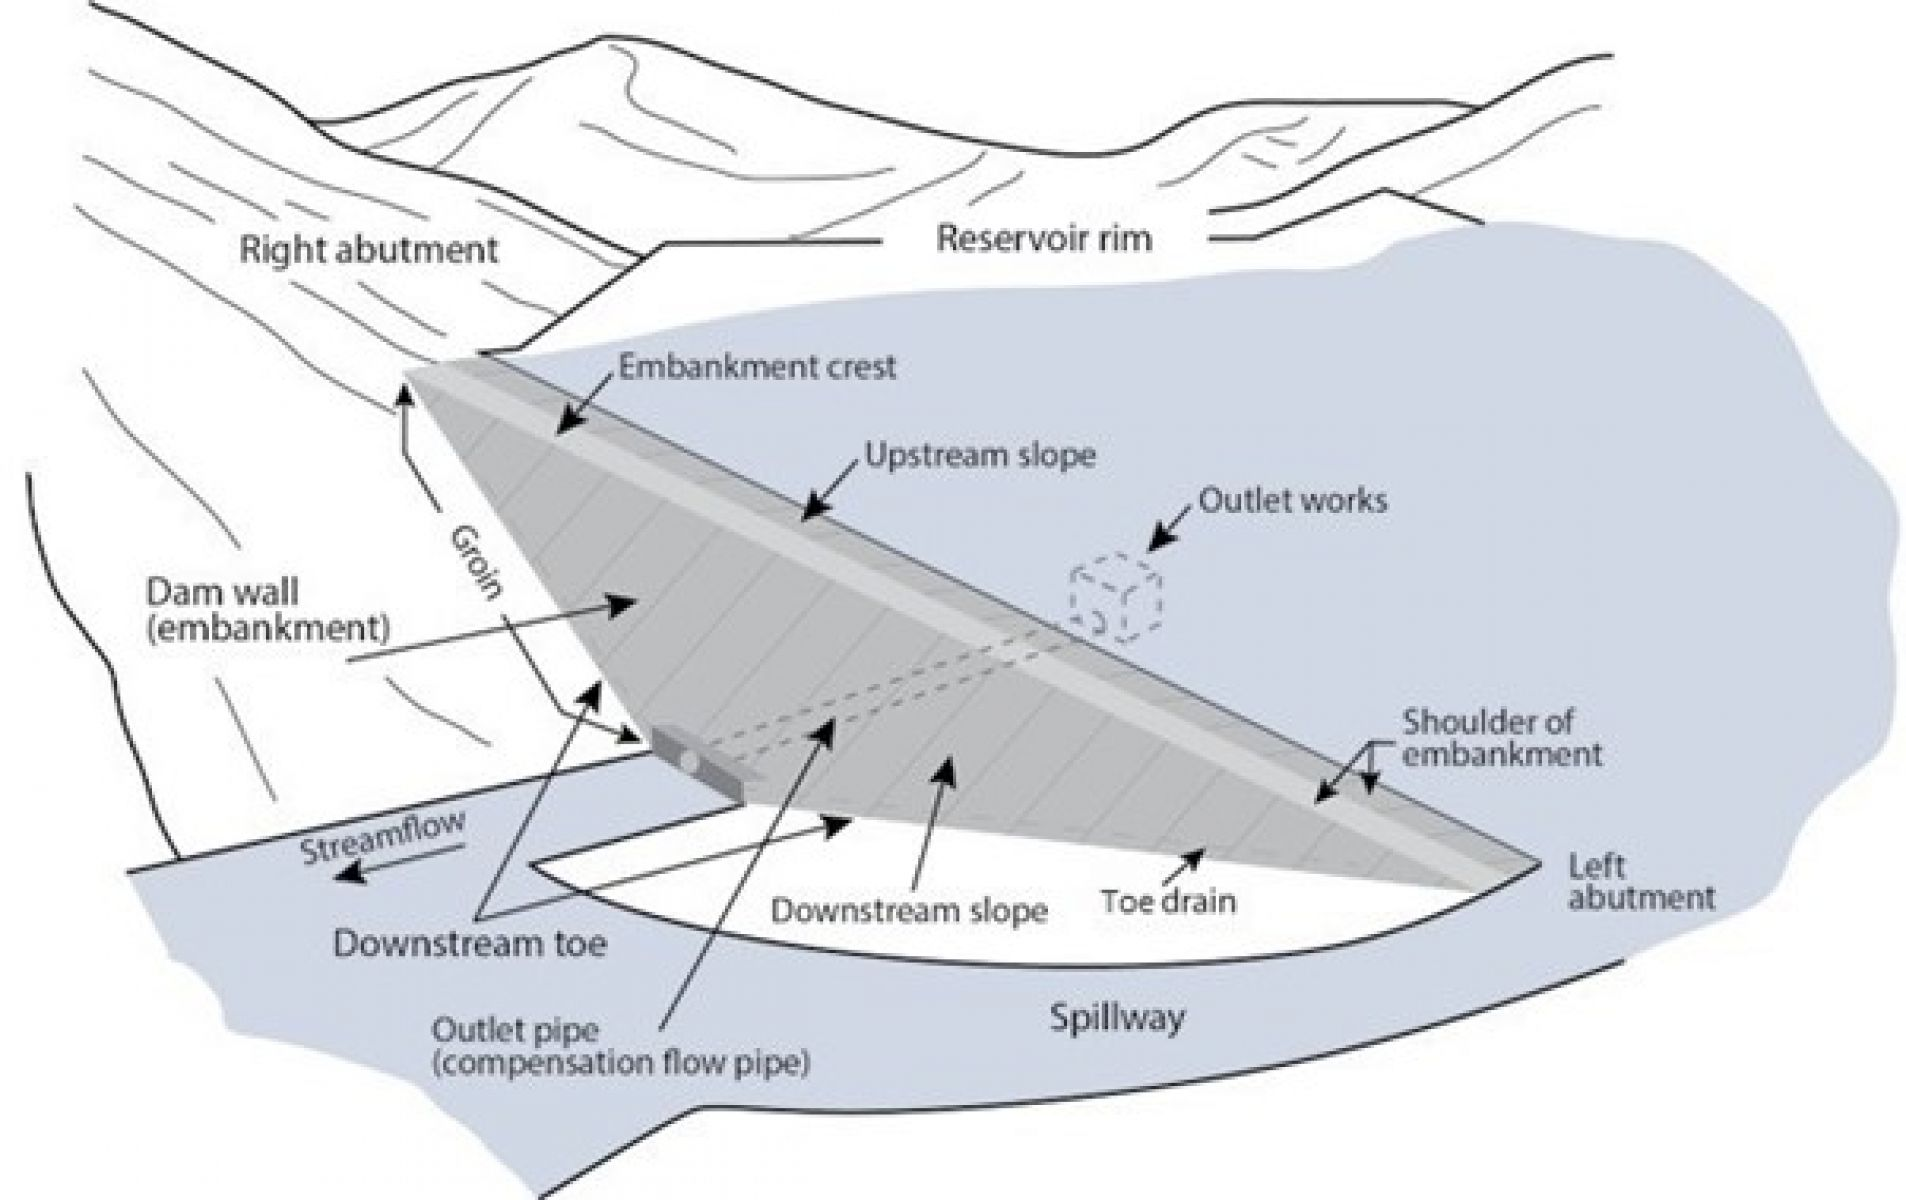
\includegraphics[width=0.8\textwidth]{Victoria_Dam_eng.jpg}
		\caption{Engineering Structures of The Victoria Dam}
		\label{fig 1:victoriadam}
	\end{figure}
	
	%=========================================
	% CHAPTER 7: NANO CONSERVATION
	%=========================================
	\chapter{Nanotechnological Applications for Heritage Conservation}
	
	\section{The Threat of Material Degradation}
	As analyzed, Sri Lanka's engineering marvels are in a state of continuous degradation. Ancient brickwork at Jetavanaramaya suffers from capillary water absorption, while concrete structures experience micro-cracking due to dynamic fatigue. Standard civil methods are inadequate, paving the way for Nano Science Technology (NANO2162) to provide sustainable solutions \cite{silva2020}.
	
	\begin{table}[H]
		\centering
		\caption{Proposed Nanomaterials for Structural Conservation}
		\label{tab:nano_materials}
		\begin{tabular}{@{}llp{6cm}@{}}
			\toprule
			\textbf{Target Structure} & \textbf{Nanomaterial Proposed} & \textbf{Primary Conservation Mechanism} \\ \midrule
			Jetavanaramaya Bricks & Nano-Silica ($SiO_2$) Suspensions & Imparts superhydrophobicity to pores. \\
			Sigiriya Frescoes & Nano-Calcium Hydroxide & Re-consolidates crumbling lime plaster. \\
			Nine Arches Mortar & Nano-Titanium Dioxide ($TiO_2$) & Photocatalytic self-cleaning and strengthening. \\
			Victoria Dam Concrete & Carbon Nanotube (CNT) Sensors & Real-time piezoresistive micro-crack detection. \\ \bottomrule
		\end{tabular}
	\end{table}
	
	\section{Nano-Silica ($SiO_2$) and the Washburn Equation}
	The primary cause of degradation in ancient bricks is water ingress. According to the Washburn equation for capillary flow:
	
	\begin{equation}
		L^2 = \frac{\gamma r t \cos(\theta)}{2 \eta}
	\end{equation}
	
	Where $L$ is penetration depth, $\gamma$ is surface tension, $r$ is pore radius, $\eta$ is viscosity, and $\theta$ is the contact angle. 
	
	\begin{figure}[H]
		\centering
		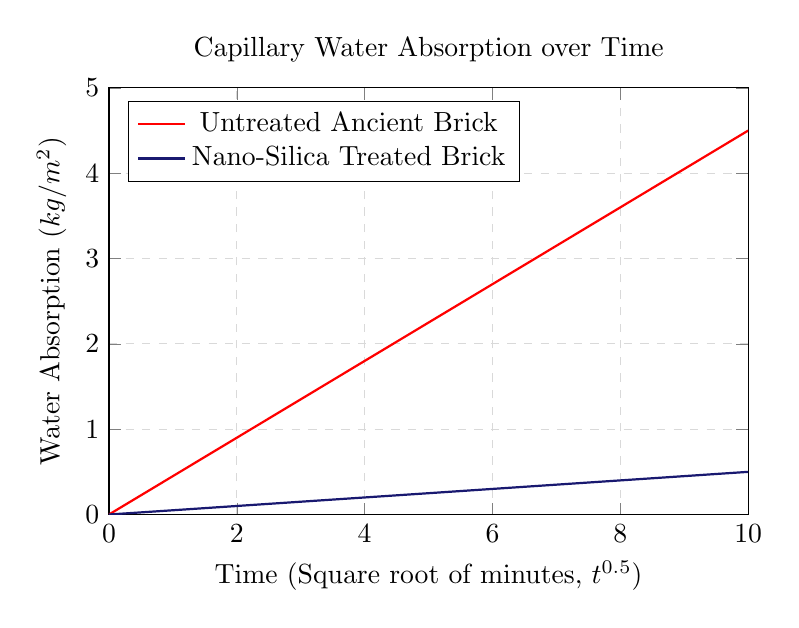
\begin{tikzpicture}
			\begin{axis}[
				width=0.8\textwidth, height=7cm,
				title={Capillary Water Absorption over Time},
				xlabel={Time (Square root of minutes, $t^{0.5}$)}, ylabel={Water Absorption ($kg/m^2$)},
				xmin=0, xmax=10, ymin=0, ymax=5,
				legend pos=north west, grid=major, grid style={dashed, gray!30},
				]
				% Untreated brick absorbs rapidly
				\addplot[color=red, thick, domain=0:10, samples=50] {0.45 * x}; 
				\addlegendentry{Untreated Ancient Brick}
				
				% Nano-silica treated brick repels water (very low slope)
				\addplot[color=MidnightBlue, thick, domain=0:10, samples=50] {0.05 * x}; 
				\addlegendentry{Nano-Silica Treated Brick}
			\end{axis}
		\end{tikzpicture}
		\caption{Applying nano-silica changes the contact angle ($\theta$) to $>90^\circ$, rendering $\cos(\theta)$ negative. This fundamentally stops capillary water absorption, protecting the structure.}
		\label{fig:capillary_action}
	\end{figure}
	
	By applying superhydrophobic nano-silica, nanoparticles penetrate deep into the microscopic pores of the bricks. They modify the surface tension, rendering the pores hydrophobic without altering the historical breathability of the artifact \cite{weerasinghe2023}.
	
	\section{Self-Healing Concrete and CNT Nano-Sensors}
	For structures like the Nine Arches Bridge and Victoria Dam, micro-cracking compromises integrity. Modern nanotech proposes the integration of encapsulated healing agents (e.g., calcium lactate and specialized bacteria). When a micro-crack forms and water enters, the capsules rupture, and the bacteria precipitate calcite, autonomously healing the crack \cite{dias2018}. 
	
	Furthermore, Carbon Nanotube (CNT) embedded sensors applied to the Victoria Dam's abutments can detect piezoresistive changes, offering real-time structural health monitoring (SHM) far more accurately than macro-scale strain gauges.
	
	%=========================================
	% CONCLUSION
	%=========================================
	\chapter{Conclusion}
	The engineering marvels of Sri Lanka are profound demonstrations of civil, structural, and geotechnical mastery. By applying rigorous mathematical modeling—from Torricelli's Law to Terzaghi's bearing capacity and hydrostatic integrations—this report has highlighted the true technical brilliance of these structures across distinct engineering disciplines. 
	
	From the dynamic deep compaction beneath the Jetavanaramaya to the double curvature optimization of the Victoria Dam, Sri Lankan engineering showcases a continuous evolution of adapting to complex environments. However, as these monuments face unprecedented environmental degradation, historical reverence alone is insufficient. As established in this report, the integration of modern Nanotechnology—such as nano-silica consolidants and self-healing matrices—is the imperative next step to ensuring the structural survival of Sri Lanka's engineering heritage for future generations.
	
	\renewcommand{\bibname}{References}
	\begin{thebibliography}{15}
		
		\bibitem{bandaranayake1974} Bandaranayake, S. (1974). \textit{Sinhalese Monastic Architecture: The Viháras of Anurádhapura}. Brill Academic Publishers.
		\bibitem{munasinghe2018} Munasinghe, D., \& Ratnayake, H. (2018). Structural Analysis of Ancient Brick Stupas: A Finite Element Approach. \textit{Journal of Archaeological Engineering}, 12(4), 45-58.
		\bibitem{senanayake2021} Senanayake, A. (2021). Hydrological Modeling and LiDAR Mapping of the Jaya Ganga Canal System. \textit{Int. Journal of Water Resources}, 29(2), 112-128.
		\bibitem{perera2014} Perera, D. (2014). \textit{The Ceylon Railway: The Story of its Inception and Growth}. Colombo Historical Society.
		\bibitem{halcrow1985} Sir William Halcrow \& Partners (1985). \textit{The Victoria Project: Design and Construction of the Victoria Dam}. Mahaweli Authority of Sri Lanka.
		\bibitem{silva2020} Silva, R., et al. (2020). Nanomaterials in Heritage Conservation: Asian Perspectives. \textit{Journal of Cultural Heritage}, 44, 215-224.
		\bibitem{ratnayake2019} Ratnayake, H., \& Fernando, S. (2019). Geotechnical Deep Compaction in Ancient Sri Lanka. \textit{Asian Geotechnical Engineering}, 18(3), 77-89.
		\bibitem{cooray1984} Cooray, P.G. (1984). \textit{An Introduction to the Geology of Sri Lanka}. National Museums of Sri Lanka.
		\bibitem{fernando2022} Fernando, M., \& Gunawardena, T. (2022). Thermodynamics of Mass Concrete in Tropical Climates: The Victoria Dam Case. \textit{Civil Eng. Journal}, 38(1), 12-25.
		\bibitem{jayawardena2017} Jayawardena, K. (2017). \textit{Hydraulic Marvels of Ancient Ceylon}. Sri Lanka Institute of Engineers.
		\bibitem{karunaratne2015} Karunaratne, P. (2015). Arch Mechanics and Material Fatigue in Colonial Railway Bridges. \textit{Journal of Structural Engineering SL}, 11(2), 55-68.
		\bibitem{weerasinghe2023} Weerasinghe, L. (2023). Nano-silica Applications for Ancient Brickwork Conservation. \textit{Nanotechnology in Construction}, 9(4), 302-315.
		\bibitem{dias2018} Dias, A., \& Mendis, P. (2018). Reservoir-Induced Seismicity in Mahaweli Dams. \textit{Geological Society Journal}, 22(1), 40-52.
		\bibitem{rajapakse2021} Rajapakse, R. (2021). Bio-inorganic Mortars in Anuradhapura: A Material Science Review. \textit{Archaeometry}, 63(3), 510-525.
		\bibitem{wijesuriya1998} Wijesuriya, G. (1998). \textit{Buddhist Monastic Architecture in Sri Lanka}. Department of Archaeology, Sri Lanka.
		
	\end{thebibliography}
	
\end{document}